%% Elsevier elsarticle template for Computers & Operations Research

\documentclass[preprint,12pt,authoryear,a4paper,fleqn]{elsarticle}

% Bibliography options - Harvard style for CAOR
% \biboptions{authoryear,longnamesfirst}
\biboptions{authoryear,longnamesfirst}
% Your packages
\usepackage{amsmath,amssymb}
\usepackage{bm}
\usepackage{algorithm}    % defines the algorithm float
\usepackage{algpseudocode}  % defines \begin{algorithmic}, \State, ...
\usepackage{float}        % (optional) for [!t] placement specifier
\usepackage{booktabs}
\usepackage{pgfplots}
\usepackage{tabularx}
\usepackage{tikz}
\usetikzlibrary{matrix,calc}
\pgfplotsset{compat=1.18}

% ---------- Theorem-like environments ----------
\usepackage{amsthm}
\newtheorem{theorem}{Theorem}
\newtheorem{lemma}[theorem]{Lemma}
\newtheorem{corollary}[theorem]{Corollary}
\theoremstyle{definition}
\newtheorem{definition}{Definition}
\newtheorem{remark}{Remark}
\newtheorem{assumption}{Assumption}
\newenvironment{pf}[1][Proof]{\begin{proof}[#1]}{\end{proof}}

\newcommand{\Occ}{\operatorname{Occ}}

\begin{document}
\let\WriteBookmarks\relax
\def\floatpagepagefraction{1}
\def\textpagefraction{.001}

\begin{frontmatter}

% Main title
\title{A Graph-Based and Metaheuristic Approach to the 2D Shortest Superstring Problem}

\author[vinuni]{Dat Thanh Tran}
\ead{dat.tt3@vinuni.edu.vn}
\author[vinuni]{Khai Quang Tran}
\ead{23khai.tq@vinuni.edu.vn}
\author[vinuni]{Van Khu Vu \corref{cor1}}
\ead{khu.vv@vinuni.edu.vn}

\cortext[cor1]{Corresponding author}

\affiliation[vinuni]{organization={VinUniversity}, city={Hanoi}, country={Vietnam}}

\begin{abstract}
We investigate a two-dimensional generalization of the Shortest Superstring Problem (SSP): given a set of 2D strings (symbol arrays), place them on the integer grid with symbol-consistent overlaps to minimize a bounding-box cost. We study two cost variants: a \emph{square} objective minimizing $\max\{H,W\}$, and an \emph{area} objective minimizing $H \cdot W$.

Our key modelling insight is to represent solutions as trees of relative offsets in a \emph{placement graph}, capturing local adjacency structure. We prove that connected placements correspond bijectively to feasible spanning trees, enabling an ILP formulation for exact solutions on small instances. Building on this structure, we develop a greedy heuristic and a tree-based genetic algorithm (GA) whose crossover preserves coherent local neighborhoods.

Experiments show that the GA matches ILP-optimal solutions on small instances and outperforms greedy by 6--12\% on larger instances, while remaining orders of magnitude faster than ILP.
\end{abstract}

\begin{keyword}
Shortest superstring problem \sep Two-dimensional strings \sep Genetic algorithm \sep Integer linear programming \sep Combinatorial optimization \sep Metaheuristics
\end{keyword}

\end{frontmatter}

% ===================== MAIN TEXT =====================

\section{Introduction}
\label{sec:intro}

The Shortest Superstring Problem (SSP) is a classical NP-hard problem~\citep{gallant1980finding}:
given a collection of strings, the goal is to construct the shortest string that
contains each input string as a contiguous substring. SSP has been extensively
studied, with known approximation algorithms~\citep{blum1994linear, mucha2013ssp} and rich connections to
combinatorial optimization and data compression.

In many modern applications, however, the objects of interest are not
one-dimensional strings but two-dimensional patterns: small images,
symbol arrays, or 2D strings. Examples include patterned fabrication, 2D barcodes,
structured-light patterns, and 2D covering sequences. Recent work has begun to
explore 2D analogues of covering and de Bruijn-type sequences, introducing the
notion of covering 2D-sequences whose windows cover all patterns of a
given size up to small Hamming radius~\citep{yehezkeally2025covering}.

In this work we study a two-dimensional generalization of the Shortest
Superstring Problem (2D-SSP), where the basic objects are rectangular
2D strings $T_1,\dots,T_n$ (finite 2D arrays over a finite alphabet), collected into a set $\mathcal{T}$. The goal is to place them
in the plane with overlaps so that all 2D strings are embedded consistently while
minimizing a bounding-box cost derived from the minimal axis-aligned bounding rectangle enclosing the occupied region. We consider two natural cost variants:
\begin{itemize}
    \item a \emph{square objective}, which minimizes the side length $\max\{H,W\}$ of the smallest enclosing square;
    \item an \emph{area objective}, which minimizes the rectangle area $H \cdot W$.
\end{itemize}

Our central modelling choice is to represent a solution as a \emph{tree of
relative offsets between 2D strings} rather than as an explicit 2D array or a vector of absolute coordinates. This choice is motivated by both theoretical and algorithmic considerations.

From a \emph{theoretical} perspective, we prove that every connected placement corresponds to a spanning tree of a naturally defined contact graph, and conversely, every feasible spanning tree induces a valid placement. This equivalence (Theorem~\ref{thm:tree-optimal}, Section~\ref{sec:problem}) shows that trees provide a complete and non-redundant encoding of the solution space.

From an \emph{algorithmic} perspective, the tree representation has a crucial advantage for metaheuristic search: it captures \emph{local structure}. Consider a good partial solution where strings $A$, $B$, and $C$ form a tightly packed cluster. In a tree representation, this cluster corresponds to a subtree, and the relative offsets within the subtree encode exactly how these strings fit together. A crossover operator can transplant this entire subtree from one parent to another, preserving the beneficial local arrangement---a principle aligned with the building block hypothesis in genetic algorithms~\citep{goldberg1989genetic}. In contrast, a coordinate-based representation stores only absolute positions $(x_A, y_A), (x_B, y_B), (x_C, y_C)$; crossover that mixes coordinates from different parents will almost certainly destroy the cluster's internal structure, since the absolute positions are meaningful only relative to a specific global arrangement.

This observation suggests that tree-based crossover should produce higher-quality offspring than coordinate-based crossover, a hypothesis confirmed by our experiments: our tree-based GA consistently outperforms greedy baselines and matches ILP-optimal solutions on small instances while scaling to much larger problems.

\section{Background and Related Work}
\label{sec:background}

\subsection{Shortest Superstring Problem}

In the classical SSP, the input is a set of strings
\[
\mathcal{S} = \{s_1,\dots,s_n\}
\]
over an alphabet \(\Sigma\). A superstring is a string \(S\) in which each
\(s_i\) appears as a substring. The objective is to minimize \(|S|\). SSP is
NP-hard, and there is a substantial literature on constant-factor
approximations (e.g., greedy maximum-overlap merging, cycle-cover-based
algorithms) and heuristic implementations used in practice.

\subsection{2D Strings and Covering Structures}

Two-dimensional generalizations of string concepts appear in several areas:
\begin{itemize}
    \item \emph{2D covers and 2D strings.} Work on covers of 2D arrays
    considers how a small pattern can cover a larger 2D string with overlaps,
    generalizing the notion of a cover in 1D~\citep{charalampopoulos2021covers}.
    \item \emph{Covering sequences and 2D covering sequences.} Recent research
    introduces covering sequences and covering 2D-sequences, where all
    $m \times n$ windows of a large 2D array form a covering code for patterns
    of that size up to a given radius. These provide natural sources of
    structured test instances~\citep{yehezkeally2025covering}.
\end{itemize}

These works focus on covering combinatorial spaces, whereas we focus on
overlapping a \emph{given finite set} of 2D strings with exact symbol consistency.

\subsection{2D Bin Packing}

Classical two-dimensional bin packing problems ask how to place a collection of
rectangles into one or more rectangular bins so as to minimize, for example,
the number of bins used or the height of a single strip, under strict
\emph{non-overlap} constraints. The items are unlabeled shapes.

Our setting is similar in that we also optimize a global bounding box for a
family of rectangular pieces, but differs in two key ways. First, each string is
a \emph{discrete symbol array} rather than an unlabeled rectangle; second,
\emph{overlaps are allowed} as long as they are \emph{symbol-consistent}. Thus a
solution is not simply a packing of shapes, but a combinatorial ``gluing'' of
patterns in which overlaps can reduce the effective occupied area, a phenomenon
absent from standard 2D bin packing.

\subsection{Related Geometric and Assembly Problems}

While 2D-SSP is distinct in its requirement for exact symbol consistency, it shares significant structural similarities with problems in VLSI design, computer graphics, and molecular computing.

In Very Large Scale Integration (VLSI) physical design, the floorplanning stage seeks to arrange rectangular modules without overlap to minimize total area and wirelength \citep{wong1986new}. This problem is a close cousin to 2D bin packing, but the methodological overlap with our work lies in the \emph{representation} of solutions. Topological representations such as Sequence Pairs \citep{murata1995sequence} and B*-trees \citep{chang2000b} encode relative positions of rectangles to explore the search space efficiently. Our use of placement trees (Section~\ref{sec:problem}) is conceptually related to these nonslicing floorplan representations, adapted to the regime where adjacency is defined by content overlap rather than physical interconnects.

In computer graphics, patch-based texture synthesis aims to generate large textures by stitching together small sample patches \citep{efros2001image, kwatra2003graphcut}. Algorithms in this domain typically place patches greedily or via graph cuts to minimize the visual error in the overlapping regions. 2D-SSP can be viewed as the discrete, lossless limit of these problems: instead of minimizing a pixel-difference norm (soft constraint), we require zero Hamming distance in the overlap (hard constraint) and optimize for maximum compression.

The constraints of 2D-SSP strongly resemble the algorithmic self-assembly of DNA tiles. In the Tile Assembly Model (TAM) introduced by \citet{winfree1998algorithmic}, square tiles (Wang tiles) attach to a growing crystal lattice only if their edges match the specific "sticky ends" (symbols) of neighbors. While DNA self-assembly focuses on the forward kinetic process of crystallization or the computational power of the resulting tiling, 2D-SSP effectively asks for the most compact configuration (or "seed") that could theoretically be assembled from a given multiset of patterned tiles.

2D-SSP can also be viewed through the lens of computational jigsaw puzzle assembly, where the goal is to reconstruct an image from a set of pieces based on visual compatibility at boundaries \citep{sholomon2013genetic}. In our setting, the "pieces" are 2D strings and the compatibility constraint is exact symbol matching rather than visual similarity. A key difference is that in classical jigsaw puzzles each piece has a unique location, whereas in 2D-SSP multiple valid placements may exist and the objective is to minimize the bounding box rather than reconstruct a known target. The problem also relates to polyomino packing \citep{golomb1994polyominoes}, which asks whether a given set of polyomino shapes can tile a region. However, polyomino packing typically assumes non-overlapping pieces with geometric interlocking, while 2D-SSP permits symbol-consistent overlaps that effectively "merge" the content of multiple strings---a feature that enables compression beyond what pure geometric packing allows.

\section{Problem Definition and Structural Properties}
\label{sec:problem}

We now formalize the Two-Dimensional Shortest Superstring Problem (2D-SSP), introduce the two objective variants, and develop the structural results underlying our tree-based representation. 

\subsection{Preliminaries and notation}

Let $\Sigma$ be a finite alphabet over which the 2D strings are defined. A \emph{2D-string} over $\Sigma$ is a finite
$m \times n$ array $T \in \Sigma^{m \times n}$, for some $m,n \in \mathbb{N}$.
For indices $1 \le i \le j \le m$ and $1 \le i' \le j' \le n$, we write
$T[i..j,\, i'..j']$ for the corresponding subarray and call this a
\emph{2D-substring} of $T$.

We identify a 2D string $T$ with a function on a finite index set
$C_T \subset \mathbb{Z}^2$, its set of \emph{local cell coordinates}.
We write cells as pairs $(u,v)\in\mathbb{Z}^2$ and use the same coordinate
system for both local and global positions: a translation by an offset
$p(i) = (x_i,y_i)$ sends a local cell $(u,v)$ of $T_i$ to the global cell
$p(i) + (u,v) = (x_i + u,\, y_i + v)$.
The choice of which axis is drawn horizontally or vertically is irrelevant
for our arguments; we only rely on coordinate-wise addition in $\mathbb{Z}^2$.

Let $P$ be an $m' \times n'$ 2D-string. We denote the set of its occurrences in
$T$ by
\[
\operatorname{Occ}(P,T) = \{(i,j) : T[i..i+m'-1,\; j..j+n'-1] = P\}.
\]

We will derive cost functions from the dimensions of the minimal axis-aligned
bounding rectangle of a placement, and consider two variants:
one that minimizes the area and one that minimizes the side length of the smallest enclosing square.

\subsection{Formal problem definition}

\begin{definition}\label{def:2d-superstring}
Let $\mathcal{T} = \{T_1,\dots,T_n\}$ be a finite multiset of 2D strings over
$\Sigma$, which we call \emph{2D strings}. An $m \times n$ 2D-string $S$ is a
\emph{2D-superstring} of $\mathcal{T}$ if each string $T_i$ occurs as a
2D-substring of $S$, i.e.,
\[
    \operatorname{Occ}(T_i, S) \neq \emptyset
    \quad \text{for all } i \in \{1,\dots,n\}.
\]
We denote by
\[
    |S|_{\mathrm{area}} := m \cdot n
    \quad\text{and}\quad
    |S|_{\square} := \max\{m,n\}
\]
the \emph{area} and the \emph{square side length} of $S$, respectively.
Both are derived from the minimal axis-aligned rectangle containing $S$ and
penalize any empty cells inside that rectangle.
\end{definition}

Thus $|S|_{\mathrm{area}}$ is the natural 2D analogue of superstring length
(area of the bounding box), while $|S|_{\square}$ focuses on the longest side
of the enclosing square.

\begin{figure}[t]
\centering
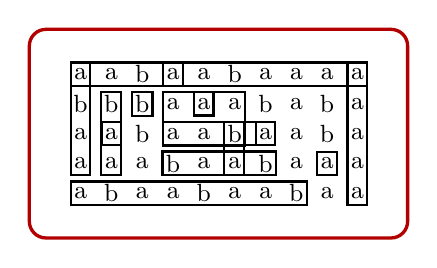
\begin{tikzpicture}[
  letter/.style={font=\small, inner sep=1pt},
  tile/.style={draw,thick},
]

%--- grid of letters ----------------------------------------------------
\matrix (m) [matrix of nodes,
  nodes in empty cells,
  nodes={letter,minimum width=0.5em,minimum height=0.8em,anchor=center},
  column sep=0.4em,row sep=0.25em
]{
  a & a & b & a & a & b & a & a & a & a \\
  b & b & b & a & a & a & b & a & b & a \\
  a & a & b & a & a & b & a & a & b & a \\
  a & a & a & b & a & a & b & a & a & a \\
  a & b & a & a & b & a & a & b & a & a \\
};

%--- outer bounding box -------------------------------------------------
\draw[very thick,rounded corners=6pt,red!70!black]
  ($(m.north west)+(-0.4,0.3)$) rectangle
  ($(m.south east)+(0.4,-0.3)$);

%--- some example tiles (rectangles over the grid) ----------------------
% long horizontal
\draw[tile] (m-1-1.north west) rectangle (m-1-10.south east);
\draw[tile] (m-5-1.north west) rectangle (m-5-8.south east);

% long vertical
\draw[tile] (m-1-1.north west) rectangle (m-4-1.south east);
\draw[tile] (m-1-10.north west) rectangle (m-5-10.south east);

% medium / short tiles
\draw[tile] (m-2-2.north west) rectangle (m-4-2.south east);
\draw[tile] (m-2-4.north west) rectangle (m-3-6.south east);
\draw[tile] (m-3-4.north west) rectangle (m-3-7.south east);
\draw[tile] (m-4-4.north west) rectangle (m-4-7.south east);
\draw[tile] (m-3-6.north west) rectangle (m-4-6.south east);

% some 1x1 tiles
\foreach \r/\c in {1/4,2/3,2/5,3/2,3/7,4/9}{
  \draw[tile] (m-\r-\c.north west) rectangle (m-\r-\c.south east);
}

\end{tikzpicture}
\caption{Example of a 2D-superstring with multiple 2D strings placed on a grid. Each rectangle indicates a 2D string; overlapping regions share identical symbols.}
\label{fig:2d-superstring-example}
\end{figure}

\begin{definition}
Given a finite multiset $\mathcal{T}$ of 2D strings over $\Sigma$, we define two
variants of the Two-Dimensional Shortest Superstring Problem:
\begin{itemize}
    \item \emph{Area-based 2D-SSP} (2D-SSP$_{\mathrm{area}}$): find a 2D-superstring $S$ of $\mathcal{T}$ minimizing $|S|_{\mathrm{area}}$.
    \item \emph{Square-based 2D-SSP} (2D-SSP$_{\square}$): find a 2D-superstring $S$ of $\mathcal{T}$ minimizing $|S|_{\square}$.
\end{itemize}
Both objectives depend only on the minimal axis-aligned bounding rectangle of $S$ and penalize all empty cells inside it.
\end{definition}

Whenever the distinction between the two variants is not important, we simply refer to either as \emph{2D-SSP}. Hereafter, we use \emph{string} to mean \emph{2D string} unless otherwise specified.

We assume throughout that strings are axis-aligned rectangles and cannot be
rotated or reflected; repeated strings in $\mathcal{T}$ are treated as distinct
objects that must each be embedded at least once.

\subsection{Placements and symbol consistency}

Rather than working directly with the superstring $S$, we use placements on the integer grid.

\begin{definition}
A \emph{placement} of $\mathcal{T}$ is a function
\[
    p : \{1,\dots,n\} \to \mathbb{Z}^2, \qquad p(i) = (x_i,y_i),
\]
assigning an integer offset to each string $T_i$. A cell of $T_i$ with local
coordinates $(u,v)$ (row and column indices) is mapped to global coordinates
$(x_i + u,\, y_i + v) \in \mathbb{Z}^2$.
\end{definition}

A placement $p$ is symbol-consistent if for every global coordinate $(x,y) \in \mathbb{Z}^2$, all strings covering $(x,y)$ under $p$ write the same symbol. We denote by
\[
\begin{aligned}
R(p) := \{(x,y) \in \mathbb{Z}^2 :\;
    & (x,y) \text{ is covered by some } T_i  \\
    & \text{under } p \}
\end{aligned}
\]
the union of occupied global cells, and let $B(p)$ be the minimal
axis-aligned rectangle containing $R(p)$. Let $W(p)$ and $H(p)$ be the width and height of $B(p)$, and define
\[
  \mathrm{cost}_{\mathrm{area}}(p) := W(p)\cdot H(p),
  \qquad
  \mathrm{cost}_{\square}(p) := \max\{W(p),H(p)\}.
\]
Restricting the symbol map to $B(p)$ yields an $m \times n$ array $T_p$; by construction $T_p$ is a 2D-superstring of $\mathcal{T}$, and its area and square side satisfy
\[
|T_p|_{\mathrm{area}} = \mathrm{cost}_{\mathrm{area}}(p),
\qquad
|T_p|_{\square} = \mathrm{cost}_{\square}(p).
\]

In particular, empty cells of $B(p)$ that are not covered by any strings still contribute to both objectives.
Thus every symbol-consistent placement defines a feasible solution to both 2D-SSP$_{\mathrm{area}}$ and 2D-SSP$_{\square}$, with cost equal to the chosen bounding-box functional.

Conversely, let $S$ be a 2D-superstring of $\mathcal{T}$ and fix
an arbitrary occurrence $(i,j) \in \operatorname{Occ}(T_k,S)$ for each string $T_k$.
Placing $T_k$ with offset $(i,j)$ then yields a symbol-consistent
placement whose induced array is $S$ up to a global translation.
Hence optimizing over 2D-superstrings is equivalent to optimizing
over symbol-consistent placements, modulo a global shift of all
coordinates.  We therefore work with placements from now on.

\subsection{Contact graphs and connectivity}

We now focus on connected placements, which is the regime of interest
for our applications and structural results; this is formalized in
Assumption~\ref{ass:connected-union} below.

A subset $R \subseteq \mathbb{Z}^2$ is \emph{4-connected} if its adjacency graph
under the 4-neighbourhood ($\|x-y\|_1 = 1$) is connected. Two cells
$x,y\in\mathbb{Z}^2$ overlap if $x=y$.

\begin{definition}
Let $p$ be a symbol-consistent placement of $\mathcal{T}$. The
\emph{contact graph} $G^{\mathrm{ct}}(p)$ is the graph with vertex set
$\{1,\dots,n\}$, where two distinct strings $i$ and $j$ are adjacent if either
\begin{itemize}
    \item $T_i$ and $T_j$ have non-empty symbol-consistent overlap under $p$, or
    \item There exist global cells $x$ of $T_i$ and $y$ of $T_j$ with
          $\|x-y\|_1 = 1$ (that is, $x$ and $y$ are 4-adjacent).
\end{itemize}

In other words, an edge of $G^{\mathrm{ct}}(p)$ records that $T_i$ and
$T_j$ touch in the final arrangement, either by overlapping or by sharing a
side.

\end{definition}

\begin{remark}
Our cost functionals depend only on the bounding rectangle $B(p)$, not directly on the cardinality of $R(p)$. In particular, two placements with the same bounding box have the same cost for both 2D-SSP$_{\mathrm{area}}$ and 2D-SSP$_{\square}$. This choice mirrors the 1D shortest superstring objective (string length) in the area-based case and a natural ``square'' version in the other case, and differs from geometric covering formulations that minimize the area of the union $R(p)$.
\end{remark}

\begin{assumption}[Connectivity of optimal unions]
\label{ass:connected-union}
In the structural discussion below we restrict attention to instances
for which there exists an optimal symbol-consistent placement $p^\ast$
(minimizing either $\mathrm{cost}_{\mathrm{area}}$ or $\mathrm{cost}_{\square}$)
whose occupied region $R(p^\ast)$ is
4-connected.
\end{assumption}

The following lemma shows that this assumption is without loss of generality: any optimal placement that is not 4-connected can be transformed into a 4-connected optimal placement.

\begin{lemma}
\label{lem:make-connected}
Let $p$ be an optimal symbol-consistent placement for 2D-SSP (under either $\mathrm{cost}_{\mathrm{area}}$ or $\mathrm{cost}_{\square}$). If $R(p)$ is not 4-connected, then there exists an optimal symbol-consistent placement $p'$ such that $R(p')$ is 4-connected and $\mathrm{cost}(p') \le \mathrm{cost}(p)$.
\end{lemma}

\begin{pf}
Suppose $R(p)$ is not 4-connected. Then the occupied region decomposes into $k \geq 2$ maximal 4-connected components $R_1, R_2, \ldots, R_k$. Each component $R_\ell$ corresponds to a subset $\mathcal{T}_\ell \subseteq \mathcal{T}$ of strings whose footprints are entirely contained in $R_\ell$. Let $B_\ell$ denote the axis-aligned bounding box of $R_\ell$, with width $W_\ell$ and height $H_\ell$.

We construct $p'$ by translating the components to merge them while ensuring their bounding boxes become adjacent without interpenetration. Without loss of generality, consider merging $R_2$ into the region containing $R_1$. Let
\begin{align*}
  x_1^{\max} &= \max\{x : (x,y) \in B_1 \text{ for some } y\}, \\
  x_2^{\min} &= \min\{x : (x,y) \in B_2 \text{ for some } y\}.
\end{align*}
We choose the translation vector $\tau = (x_1^{\max} - x_2^{\min} + 1, \delta_y)$, where:
\begin{itemize}
    \item The horizontal component $x_1^{\max} - x_2^{\min} + 1$ is the unique value that places the leftmost column of the translated $B_2$ immediately to the right of the rightmost column of $B_1$, ensuring the two bounding boxes are horizontally adjacent but do not overlap.
    \item The vertical component $\delta_y$ is chosen to ensure vertical overlap: if the $y$-projections of $B_1$ and $B_2$ already intersect, we set $\delta_y = 0$; otherwise, we set $\delta_y$ to the minimum shift needed to make them share at least one row.
\end{itemize}
This construction guarantees that the translated $B_2$ and $B_1$ share a common edge (or at least a corner), making the combined region 4-connected.

We now verify that:
\begin{enumerate}
    \item \emph{Symbol-consistency is preserved.} Before translation, strings in $\mathcal{T}_1$ and $\mathcal{T}_2$ had no overlapping cells (since $R_1$ and $R_2$ were disjoint). After translation, the bounding boxes $B_1$ and the translated $B_2$ are adjacent but non-overlapping by construction of $\tau$. Therefore, no cell can be occupied by both a string from $\mathcal{T}_1$ and a string from $\mathcal{T}_2$, and no symbol conflict arises. Symbol-consistency within each $\mathcal{T}_\ell$ is trivially preserved since internal offsets are unchanged.
    
    \item \emph{The bounding box dimensions do not increase (for either cost variant).} Let $B(p) = [x_{\min}, x_{\max}] \times [y_{\min}, y_{\max}]$ with width $W = x_{\max} - x_{\min} + 1$ and height $H = y_{\max} - y_{\min} + 1$. 
    
    \emph{Key observation:} Both cost functions $\mathrm{cost}_{\mathrm{area}}(p) = W \cdot H$ and $\mathrm{cost}_{\square}(p) = \max(W, H)$ are \emph{monotonically increasing} in each dimension. Equivalently, they are monotonically decreasing with respect to the removal of empty space from the bounding box. Since the components $R_1, \ldots, R_k$ are pairwise disjoint and all fit within $B(p)$, there must exist gaps (empty columns or rows) separating them within $B(p)$---otherwise they would not be disconnected. Our translation removes these gaps.
    
    After merging $R_1$ and $R_2$ horizontally, denote the new bounding box dimensions by $W'$ and $H'$. We have:
    \begin{itemize}
        \item $W' = W_1 + W_2 \le W - 1 < W$: the strict inequality holds because $B_1$ and $B_2$ originally fit within $[x_{\min}, x_{\max}]$ with at least one empty column between them (the gap that separated the disconnected components).
        \item $H' = \max(H_1, H_2) \le H$: the height of the merged region is the maximum of the two component heights, which cannot exceed the original height. If a vertical shift $\delta_y \neq 0$ was applied, it can only decrease $H'$ further (by aligning the components vertically).
    \end{itemize}
    
    Since $W' < W$ and $H' \le H$, we have coordinate-wise strict improvement in at least one dimension:
    \begin{align*}
        \mathrm{cost}_{\mathrm{area}}(p') &= W' \cdot H' < W \cdot H = \mathrm{cost}_{\mathrm{area}}(p), \\
        \mathrm{cost}_{\square}(p') &= \max(W', H') \le \max(W, H) = \mathrm{cost}_{\square}(p).
    \end{align*}
    The area inequality is strict; the square inequality may be an equality (if the original $\max$ was determined by $H$ and $H' = H$), but in no case does the cost increase.
\end{enumerate}

Repeating this process for all remaining components yields a placement $p'$ with $R(p')$ 4-connected and $\mathrm{cost}(p') \le \mathrm{cost}(p)$. Since $p$ was optimal, we have $\mathrm{cost}(p') = \mathrm{cost}(p)$, so $p'$ is also optimal.
\end{pf}

\begin{corollary}
For any instance of 2D-SSP, there exists an optimal placement whose occupied region is 4-connected. Consequently, Assumption~\ref{ass:connected-union} holds for all instances.
\end{corollary}

This structural result justifies our focus on connected placements: rather than being a restrictive modelling choice, connectivity is a property that can always be achieved at optimality. The assumption matches our experimental
focus and enables the tree-based structural perspective developed in this section. It is not required for the correctness of the algorithms in
Section~\ref{sec:algorithms}, which operate on arbitrary
symbol-consistent placements.

\begin{lemma}
\label{lem:contact-connected}
Let $p$ be a symbol-consistent placement such that $R(p)$ is 4-connected.
Then the contact graph $G^{\mathrm{ct}}(p)$ is connected.
\end{lemma}

\begin{pf}
If $G^{\mathrm{ct}}(p)$ were disconnected, we could partition the strings into
two nonempty sets $A$ and $B$ with no edge between them. For each string $T_i$, let $R_i$ be the set of global cells covered by $T_i$
under $p$. Define
\[
  R_A = \bigcup_{i\in A} R_i,
  \qquad
  R_B = \bigcup_{j\in B} R_j,
\]
so that $R(p) = R_A \cup R_B$ and $R_A \cap R_B = \emptyset$.
By construction there is no pair of 4-adjacent cells across $R_A$ and $R_B$,
which contradicts 4-connectivity of $R(p)$.
\end{pf}

Under Assumption~\ref{ass:connected-union} and Lemma~\ref{lem:contact-connected},
we obtain the following.

\begin{theorem}
\label{thm:growing-optimal}
Let $\mathcal{T}$ be an instance of 2D-SSP (either 2D-SSP$_{\mathrm{area}}$ or 2D-SSP$_{\square}$) that satisfies
Assumption~\ref{ass:connected-union}, and let $p^*$ be an optimal
symbol-consistent placement (with respect to the chosen cost) whose occupied region $R(p^*)$ is 4-connected.
Then the contact graph $G^{\mathrm{ct}}(p^*)$ is connected and hence admits a
spanning tree. Equivalently, there is an ordering of the strings
$(i_1,\dots,i_n)$ such that for every $t>1$, string $i_t$ is adjacent in
$G^{\mathrm{ct}}(p^*)$ to at least one string $i_s$ with $s<t$.

One can realize $p^*$ by starting from a root string and repeatedly attaching
a new string along an edge of this tree.
\end{theorem}

\subsection{Placement graphs and placement trees}

For algorithmic purposes it is convenient to encode all symbol-consistent relative offsets between strings in a separate graph.

\begin{definition}
Given the string set $\mathcal{T}$, the \emph{placement graph} $G^{\mathrm{pl}}$
has vertex set $\{1,\dots,n\}$. Its edges are triples
\[
    e = (i,j,\delta) \quad\text{with}\quad i \neq j,\; \delta \in \mathbb{Z}^2,
\]
where $\delta$ is a relative offset such that placing $T_j$ at position
$p(j) = p(i) + \delta$ is symbol-consistent with $T_i$ on their overlapping
region. In practice, we restrict to offsets that yield non-empty overlap or
4-adjacent contact; multiple offsets may exist for the same unordered pair
$\{i,j\}$.
\end{definition}

Intuitively, each edge $(i,j,\delta)$ in $G^{\mathrm{pl}}$ specifies a way of
gluing $T_j$ next to $T_i$. We represent global placements as trees of such
relative offsets.

\begin{definition}\label{def:placement-tree}
A \emph{placement tree} for $\mathcal{T}$ is a rooted tree
$F = (V,E)$ with vertex set $V = \{1,\dots,n\}$ together with, for each
edge $\{i,j\} \in E$, a label $\delta_{ij} \in \mathbb{Z}^2$ interpreted as
the relative offset from $i$ to $j$.
For each oriented edge $(i,j)$ we store $\delta_{ij}$ and require
$\delta_{ji} = -\delta_{ij}$.
\end{definition}

Fix a root $r \in V$.
For a vertex $i\in V$, let
\[
  r = v_0, v_1,\dots,v_\ell = i
\]
be the unique simple path from $r$ to $i$ in $F$.

\begin{definition}\label{def:realization}
The \emph{realization} of a placement tree $F$ with root position
$p(r)\in\mathbb{Z}^2$ is the placement $p_F$ defined by
\[
  p_F(i)
  \;=\;
  p(r) + \sum_{t=0}^{\ell-1} \delta_{v_t v_{t+1}}
  \qquad\text{for all } i \in V,
\]
where $r = v_0,\dots,v_\ell = i$ is the unique simple path from $r$ to $i$ in $F$.

We call $F$ \emph{feasible} if, for one (equivalently, for every) choice of
root position $p(r)$, the realization $p_F$ is symbol-consistent.
In this case we also refer to $p_F$ as a \emph{tree-induced placement}.
\end{definition}

\begin{remark}\label{rem:feasibility-conditions}
Feasibility is a global property of the realized coordinates: even if all
adjacent pairs $(i,j)$ are locally consistent, collisions may occur between
distant parts of the tree when their footprints overlap after summing the
offsets. We do not attempt to characterize feasibility purely in terms of local
constraints on the edge labels $(\delta_{ij})$. In particular, closed walks
in the underlying contact graph induce non-trivial ``loop-closure''
constraints on the offsets, which are difficult to express compactly.
Instead, feasibility is treated as an algorithmic property: given a placement
tree $F$, we realize it via $p_F$ and explicitly check symbol-consistency of
the resulting placement.
\end{remark}

\subsection{Structural theorems: equivalence of placements and trees}

We now formalize the correspondence between connected placements and feasible
placement trees.

\begin{lemma}
\label{lem:placement-to-tree}
Let $p$ be a symbol-consistent placement of $\mathcal{T}$ such that $R(p)$ is
4-connected, and let $G^{\mathrm{ct}}(p)$ be its contact graph. Fix any
spanning tree $F$ of $G^{\mathrm{ct}}(p)$ and choose a root $r \in V(F)$.

For each oriented edge $(i,j)$ of $F$, define
\[
    \delta_{ij} := p(j) - p(i) \in \mathbb{Z}^2.
\]
Then:
\begin{enumerate}
    \item The labeled tree $F$ is a feasible placement tree.
    \item For any choice of $p(r)$, the realization $p_F$ coincides with $p$
          up to a global translation.
\end{enumerate}
\end{lemma}

\begin{pf}
By definition of the labels, for every edge $(i,j)$ the placement $p$
satisfies $p(j) = p(i) + \delta_{ij}$.
Consequently, for any vertex $i$ and any path $r=v_0,\dots,v_\ell=i$ in $F$,
we have
\[
  p(i)
  \;=\;
  p(r) + \sum_{t=0}^{\ell-1} \delta_{v_t v_{t+1}}.
\]
Thus $p$ is a realization of $F$ for the particular choice of root position
$p(r)$.
Since $p$ is symbol-consistent, this shows that $F$ is feasible.
Changing $p(r)$ to $p(r)+\Delta$ for some $\Delta \in \mathbb{Z}^2$ adds
$\Delta$ to all positions, yielding a global translation of $p$.
\end{pf}

\begin{lemma}
\label{lem:tree-to-placement}
Let $F$ be a feasible placement tree for $\mathcal{T}$, and let $p_F$ be any
realization (for some choice of root and root position). Then $p_F$ is a
symbol-consistent placement whose induced array $T_{p_F}$ is a 2D-superstring
of $\mathcal{T}$.
\end{lemma}

\begin{pf}
By feasibility, the realization $p_F$ is symbol-consistent.
Every string $T_i$ is placed exactly once, so $T_i$ occurs as a 2D substring
of the induced array $T_{p_F}$.
Therefore $T_{p_F}$ is a 2D-superstring of $\mathcal{T}$.
\end{pf}

Combining Assumption~\ref{ass:connected-union} with
Lemmas~\ref{lem:contact-connected},
\ref{lem:placement-to-tree}, and~\ref{lem:tree-to-placement}, we obtain:

\begin{theorem}
\label{thm:tree-optimal}
Let $p$ be a symbol-consistent placement of $\mathcal{T}$ whose occupied
region $R(p)$ is 4-connected, and let $G^{\mathrm{ct}}(p)$ be its contact
graph. Then any spanning tree $F$ of $G^{\mathrm{ct}}(p)$, equipped with edge
labels
\[
  \delta_{ij} \;:=\; p(j) - p(i)
\]
for each oriented edge $(i,j)$ of $F$, is a feasible placement tree whose
realization $p_F$ coincides with $p$ up to a global translation.

Conversely, any feasible placement tree $F$ induces a symbol-consistent
placement $p_F$ and hence a feasible solution to 2D-SSP (under either bounding-box objective), with objective value
given by $\mathrm{cost}_{\mathrm{area}}(p_F)$ in the area-based variant or
$\mathrm{cost}_{\square}(p_F)$ in the square-based variant.
\end{theorem}

\begin{remark}
All lemmas and theorems in this section concern only symbol-consistency,
connectivity, and the combinatorial structure of placements. They do not use
any specific property of the cost functional beyond the fact that it is
derived from the bounding box $B(p)$. Consequently, the structural statements
apply verbatim to both 2D-SSP$_{\mathrm{area}}$ and 2D-SSP$_{\square}$.
\end{remark}

Theorem~\ref{thm:tree-optimal} establishes that placement trees provide a complete encoding of connected placements, but the theorem's value extends beyond mere equivalence. The tree structure has three properties that make it particularly suitable for metaheuristic optimization:

\begin{enumerate}
    \item \emph{Locality preservation.} In a placement tree, strings that are geometrically close in the final arrangement are typically close in the tree (separated by few edges). This means that a subtree corresponds to a spatially coherent cluster of strings. When crossover transplants a subtree from one parent to another, it preserves the internal structure of this cluster---the relative offsets that make these strings fit together well.
    
    \item \emph{Incremental realizability.} A placement tree can be ``grown'' by adding one string at a time along tree edges, always maintaining a valid partial placement. This property directly enables our greedy construction heuristic (Section~\ref{sec:greedy-impl}) and ensures that the GA's crossover operator can incrementally build feasible offspring.
    
    \item \emph{Reduced redundancy.} Unlike coordinate-based representations where infinitely many coordinate vectors encode the same placement (differing by global translation), the tree representation is essentially unique for a given contact structure. This reduces the effective search space and avoids wasting computational effort on equivalent solutions.
\end{enumerate}

These properties motivate our choice to design a genetic algorithm whose individuals are placement trees and whose crossover operates on subtrees, rather than using a more conventional coordinate-based representation.

\begin{table}[h]
  \centering
  \small
  \caption{Summary of main notation.}
  \label{tab:notation}
  \setlength{\tabcolsep}{4pt}%
  \begin{tabularx}{\columnwidth}{@{}lX@{}}
    \toprule
    Symbol & Meaning \\
    \midrule
    $\Sigma$ & Alphabet \\
    $\mathcal{T} = \{T_1,\dots,T_n\}$ & Input set of strings \\
    $C_T \subset \mathbb{Z}^2$ & Local cell coordinates of string $T$ \\
    $P$ & Pattern 2D-string (for occurrences) \\
    $\operatorname{Occ}(P,T)$ & Set of occurrences of $P$ in $T$ \\
    $S$ & 2D-superstring of $\mathcal{T}$ \\
    $|S|_{\mathrm{area}}$ & Area of minimal bounding box of $S$ \\
    $|S|_{\square}$ & Side length of minimal enclosing square of $S$ \\
    $p(i) = (x_i,y_i)$ & Placement (offset) of string $T_i$ \\
    $R(p) \subset \mathbb{Z}^2$ & Union of occupied cells under placement $p$ \\
    $B(p)$ & Minimal axis-aligned bounding box of $R(p)$ \\
    $W(p),H(p)$ & Width and height of $B(p)$ \\
    $\mathrm{cost}_{\mathrm{area}}(p)$ & Area-based cost $W(p)H(p)$ \\
    $\mathrm{cost}_{\square}(p)$ & Square-based cost $\max\{W(p),H(p)\}$ \\
    $G^{\mathrm{ct}}(p)$ & Contact graph induced by placement $p$ \\
    $G^{\mathrm{pl}}$ & Placement graph of symbol-consistent offsets \\
    $F = (V,E)$ & Placement tree on $\{1,\dots,n\}$ \\
    $\delta_{ij} \in \mathbb{Z}^2$ & Relative offset from $i$ to $j$ in $F$ \\
    $p_F$ & Realization (tree-induced placement) of $F$ \\
    \bottomrule
  \end{tabularx}
\end{table}


\section{Algorithms}
\label{sec:algorithms}

Having established the structural foundation linking placements and trees, we now present three algorithmic approaches for solving 2D-SSP. These methods span the spectrum from exact to heuristic, offering different trade-offs between solution quality and computational cost:

\begin{itemize}
    \item An \emph{exact ILP formulation} (Section~\ref{sec:ilp-baseline}) that enumerates all candidate placements on a discrete grid and optimizes over them using mixed-integer linear programming. This approach guarantees optimal solutions but is limited to small instances.
    
    \item A \emph{greedy construction heuristic} (Section~\ref{sec:greedy-impl}) that builds placements incrementally by always choosing the locally best extension. This approach is extremely fast but may produce suboptimal solutions.
    
    \item A \emph{tree-based genetic algorithm} (Section~\ref{subsec:ga}) that represents individuals as placement trees and uses crossover operators that recombine subtrees. This approach aims to combine the quality of exact methods with the scalability of heuristics.
\end{itemize}

All three methods can be instantiated with either of the two bounding-box cost variants, 2D-SSP$_{\mathrm{area}}$ or 2D-SSP$_{\square}$.

The genetic algorithm uses placement trees rather than the more obvious coordinate-based representation (where each individual is a vector of $(x,y)$ coordinates for each string). This choice is motivated by several considerations. First, in the coordinate representation, an offspring produced by crossover rarely inherits good local structure from its parents: if parent~1 places strings $A$ and $B$ in a well-overlapping configuration, and parent~2 places strings $B$ and $C$ similarly, a crossover that takes $A$ from parent~1 and $C$ from parent~2 will likely place them far apart, destroying both favorable overlaps. In contrast, our tree-based crossover transplants entire subtrees, preserving the relative offsets among all strings in the subtree. Second, the coordinate representation is highly redundant: any global translation of a placement yields the same objective value, so the search space contains infinitely many equivalent solutions. The tree representation eliminates this redundancy by encoding only the pairwise offsets that matter. Third, the tree structure aligns naturally with the connectivity requirement: a spanning tree automatically ensures that all strings are geometrically connected, whereas the coordinate representation requires additional constraints or repair operators to enforce connectivity.

\subsection{Exact Verification via ILP}
\label{sec:ilp-baseline}

To validate the solution quality of our heuristic approaches, we formulate a direct grid-based mixed-integer linear program~\citep{wolsey1999integer}. We emphasize that this formulation is \emph{not} intended as a scalable solver for general instances, but strictly as a \emph{ground-truth oracle} for small-scale verification ($N \le 10$). This allows us to measure exactly how close our genetic algorithm comes to the global optimum.

The model works with discrete candidate placements of each 2D string on a finite grid: it enumerates a finite set of allowed origins for each 2D string, chooses exactly one origin per string, forbids symbol conflicts between strings, and then optimizes the axis-aligned bounding box enclosing all occupied cells according to the chosen objective variant.

Throughout this subsection we reuse the notation from
Section~\ref{sec:problem}. In particular, we have a finite multiset of 2D
strings $\mathcal{T} = \{T_1,\dots,T_n\}$, each represented by a finite set of
local cells $C_i \subset \mathbb{Z}^2$ and a symbol function
$T_i : C_i \to \Sigma$. For each $i$ we denote the local bounding box of $T_i$
by
\begin{align*}
  x_i^{\min} &= \min_{(u,v)\in C_i} u, &
  x_i^{\max} &= \max_{(u,v)\in C_i} u, \\
  y_i^{\min} &= \min_{(u,v)\in C_i} v, &
  y_i^{\max} &= \max_{(u,v)\in C_i} v,
\end{align*}
and its width and height by
\[
  w_i = x_i^{\max} - x_i^{\min} + 1,
  \qquad
  h_i = y_i^{\max} - y_i^{\min} + 1.
\]

We embed all strings into a common rectangular grid
$[0,W_g] \times [0,H_g] \subset \mathbb{Z}^2$, where $W_g$ and $H_g$ are derived from a greedy solution computed as a preprocessing step. Specifically, we first run the greedy heuristic (Section~\ref{sec:greedy-impl}) to obtain a feasible placement with bounding-box dimensions $W_{\text{greedy}} \times H_{\text{greedy}}$. Since any optimal solution cannot have a larger bounding box than this greedy solution, we set
\[
  W_g := W_{\text{greedy}}, \qquad H_g := H_{\text{greedy}}.
\]
This significantly reduces the number of candidate origins compared to a naive bound of $N \cdot \max_i \max\{w_i, h_i\}$.

To eliminate redundant symmetric solutions arising from translation invariance, we apply \emph{symmetry breaking}: we fix the first string $T_1$ at the origin by restricting its set of allowed origins to $\mathcal{O}_1 := \{(0,0)\}$. This constraint removes all translated copies of any given solution from the search space without affecting optimality.

For each string $i \ge 2$ we define a finite set of allowed \emph{origins}
$\mathcal{O}_i \subset \mathbb{Z}^2$ such that translating $T_i$ by $o$ keeps
all its local cells inside the global grid:
\begin{equation}
  \begin{split}
    \mathcal{O}_i \;:=\; \Bigl\{\, o = (x,y) \in \mathbb{Z}^2 \,\Big|\,
    & (x+u, y+v) \in [0,W_g]\times[0,H_g] \text{ for all } (u,v)\in C_i \Bigr\}
  \end{split}
  \label{eq:ilp-origins}
\end{equation}
Recall that $\mathcal{O}_1 = \{(0,0)\}$ by the symmetry-breaking constraint.
When $T_i$ is placed at an origin $o = (x,y)$, each local cell
$(u,v)\in C_i$ is mapped to global coordinates $(x+u,y+v)$.

Two candidate placements $(i,o)$ and $(j,o')$ are incompatible if they assign
different symbols to the same global coordinate. Formally, we precompute a
Boolean conflict indicator
\begin{equation}
  \kappa_{ijoo'} =
  \begin{cases}
    1, & \begin{aligned}[t]
           &\text{if there exist } (u,v)\in C_i,\, (u',v')\in C_j \text{ with } \\
           & (x+u,y+v) =(x'+u',y'+v') \text{ and } T_i(u,v)\neq T_j(u',v') \\
           & \text{for } o=(x,y),\,o'=(x',y'),
         \end{aligned} \\
    0, & \text{otherwise},
  \end{cases}
  \label{eq:ilp-kappa}
\end{equation}
for all $i<j$, $o\in\mathcal{O}_i$, and $o'\in\mathcal{O}_j$.
This preprocessing reduces symbol consistency to simple pairwise
constraints in the ILP.

The model uses the following variables.
\begin{itemize}
  \item For each string $i \in \{1,\dots,n\}$ and each origin
        $o\in\mathcal{O}_i$:
        \[
          b_{io} \in \{0,1\}
          \quad\text{(1 if $T_i$ is placed at origin $o$, 0 otherwise).}
        \]
  \item Integer coordinates of the global bounding box:
        \[
          X_{\min}, X_{\max}, Y_{\min}, Y_{\max} \in \mathbb{Z},
        \]
        which represent the minimum and maximum global row/column indices
        among all occupied cells.
  \item The width and height of the bounding box:
        \[
          W, H \in \mathbb{Z}_{\ge 0}.
        \]
  \item A square side variable (for the square objective):
        \[
          L \in \mathbb{Z}_{\ge 0},
        \]
        representing the side length of the smallest enclosing square.
  \item An area variable (for the area objective):
        \[
          A \in \mathbb{Z}_{\ge 0},
        \]
        used to model or approximate the bounding-box area $W\cdot H$.
\end{itemize}
In the implementation we bound these variables by a constant
\[
  M \;:=\; \max\{W_g, H_g\} + \max_i \max\{w_i,h_i\},
\]
so that $X_{\min},X_{\max},Y_{\min},Y_{\max} \in [-M,M]$ and
$W,H,L \in [0,M]$, $A \in [0,M^2]$.

Both objective variants share the following groups of constraints.

\medskip
\noindent
\emph{(i) Exactly one origin per string.}
Each 2D string must be placed at exactly one origin:
\begin{equation}
  \sum_{o\in\mathcal{O}_i} b_{io} \;=\; 1
  \qquad \forall i \in \{1,\dots,n\}.
  \label{eq:ilp-one-origin}
\end{equation}

\medskip
\noindent
\emph{(ii) No symbol conflicts.}
If two candidate placements $(i,o)$ and $(j,o')$ conflict, they cannot be
chosen simultaneously:
\begin{equation}
  b_{io} + b_{jo'} \;\le\; 1
  \quad
  \forall\, i<j,\ \forall\, o\in\mathcal{O}_i,\ \forall\, o'\in\mathcal{O}_j
  \text{ with } \kappa_{ijoo'} = 1.
  \label{eq:ilp-conflict}
\end{equation}

\medskip
\noindent
\emph{(iii) Bounding box must contain all placed strings.}
Let $o=(x,y)\in\mathcal{O}_i$ be a candidate origin for $T_i$.
If $b_{io}=1$, then the global footprint of $T_i$ is
\[
  [x + x_i^{\min},\, x + x_i^{\max}]
  \times
  [y + y_i^{\min},\, y + y_i^{\max}],
\]
and this rectangle must lie inside
$[X_{\min},X_{\max}]\times[Y_{\min},Y_{\max}]$.
We encode these implications with big-$M$ constraints:
\begin{align}
  X_{\min} &\;\le\; x + x_i^{\min} + M(1-b_{io}),
  \label{eq:ilp-Xmin} \\
  X_{\max} &\;\ge\; x + x_i^{\max} - M(1-b_{io}),
  \label{eq:ilp-Xmax} \\
  Y_{\min} &\;\le\; y + y_i^{\min} + M(1-b_{io}),
  \label{eq:ilp-Ymin} \\
  Y_{\max} &\;\ge\; y + y_i^{\max} - M(1-b_{io}),
  \label{eq:ilp-Ymax}
\end{align}
for all $i$ and all $o=(x,y)\in\mathcal{O}_i$.
When $b_{io}=1$ these reduce to the desired inequalities
$X_{\min}\le x+x_i^{\min}$, $X_{\max}\ge x+x_i^{\max}$, etc., and when
$b_{io}=0$ they are relaxed by the big-$M$ terms.

\medskip
\noindent
\emph{(iv) Definition of width and height.}
The bounding box dimensions are defined by
\begin{equation}
  W = X_{\max} - X_{\min} + 1,
  \qquad
  H = Y_{\max} - Y_{\min} + 1.
  \label{eq:ilp-WH}
\end{equation}
In addition, $W$ and $H$ must be at least as large as the widest and tallest
individual 2D string:
\begin{equation}
  W \;\ge\; \max_i w_i,
  \qquad
  H \;\ge\; \max_i h_i.
  \label{eq:ilp-WH-lb}
\end{equation}

\subsubsection{Square Objective}
The square-based variant minimises the side length of the smallest enclosing square. We link $L$ to $W$ and $H$ via
\begin{equation}
  L \;\ge\; W,
  \qquad
  L \;\ge\; H.
  \label{eq:ilp-square-L}
\end{equation}
At optimality, $L = \max\{W,H\}$.

The \emph{bounding square} ILP is
\begin{align}
  \min \quad & L
  \label{eq:ilp-square-obj} \\
  \text{s.t.} \quad
  &\eqref{eq:ilp-one-origin} - \eqref{eq:ilp-WH-lb},\ \eqref{eq:ilp-square-L}, \nonumber \\
  &b_{io} \in \{0,1\}\ \forall i,o,\quad
   X_{\min},X_{\max},Y_{\min},Y_{\max},W,H,L \in \mathbb{Z}. \nonumber
\end{align}

\subsubsection{Area Objective}
The area-based variant uses the product $W\cdot H$ as its cost. Conceptually we want
\begin{equation}
  A = W \cdot H.
  \label{eq:ilp-area-ideal}
\end{equation}
To remain within a ILP framework we linearize this product over a known box
$W \in [W_{\min},W_{\max}]$, $H \in [H_{\min},H_{\max}]$.
We take
\[
  W_{\min} := \max_i w_i,\quad
  H_{\min} := \max_i h_i,\quad
  W_{\max},H_{\max} \le M,
\]
and impose the standard McCormick envelope
\begin{align}
  A &\;\ge\; W_{\min} H + H_{\min} W - W_{\min} H_{\min},
  \label{eq:ilp-mcc-1} \\
  A &\;\ge\; W_{\max} H + H_{\max} W - W_{\max} H_{\max},
  \label{eq:ilp-mcc-2} \\
  A &\;\le\; W_{\min} H + H_{\max} W - W_{\min} H_{\max},
  \label{eq:ilp-mcc-3} \\
  A &\;\le\; W_{\max} H + H_{\min} W - W_{\max} H_{\min}.
  \label{eq:ilp-mcc-4}
\end{align}
These constraints define the convex hull of all triples
$(W,H,A)$ with $A=W\cdot H$ and $(W,H)$ in the given box.
On small instances one can further tighten this relaxation by
introducing a discrete piecewise-linear approximation of $W\cdot H$,
but the simple McCormick envelope above already proved sufficient
for our experiments.

The \emph{bounding area} ILP is
\begin{align}
  \min \quad & A
  \label{eq:ilp-area-obj} \\
  \text{s.t.} \quad
  &\eqref{eq:ilp-one-origin} - \eqref{eq:ilp-WH-lb},\ \eqref{eq:ilp-mcc-1} - \eqref{eq:ilp-mcc-4}, \nonumber \\
  &b_{io} \in \{0,1\}\ \forall i,o,\quad
   X_{\min},X_{\max},Y_{\min},Y_{\max},W,H,A \in \mathbb{Z}. \nonumber
\end{align}
The objective value $A^\star$ coincides with the
area of the minimal axis-aligned bounding rectangle $B(p)$ enclosing all
occupied cells in the induced placement $p$.

\medskip
This formulation is conceptually straightforward: each $b_{io}$ encodes
a specific choice of origin for string $T_i$; the conflict constraints
\eqref{eq:ilp-conflict} enforce symbol consistency; the big-$M$
constraints \eqref{eq:ilp-Xmin}--\eqref{eq:ilp-Ymax} define a global
bounding box that contains all chosen placements; and depending on the variant,
either \eqref{eq:ilp-square-L} or
\eqref{eq:ilp-mcc-1}--\eqref{eq:ilp-mcc-4} expresses the chosen cost. The greedy-based grid bounds and symmetry breaking significantly reduce the search space, but the number of variables and conflict constraints still grows quickly with the number of strings. Consequently, this ILP is practically limited to small instances ($N \le 10$) and serves exclusively as a verification tool to certify the optimality gap of our heuristic methods.

\subsection{Greedy Heuristics}
\label{sec:greedy-impl}

We also use greedy construction heuristics that build a placement incrementally
on a global \emph{canvas}. Strings are placed one by one, always maintaining symbol-consistency and trying to keep the current bounding-box cost (either side length $\max\{\text{width},\text{height}\}$ for the square objective or area $\text{width}\times\text{height}$ for the area objective)
as small as possible. All variants start from a chosen ``root'' string and then attach the remaining strings.

Conceptually, the current solution is represented by:
\begin{itemize}
    \item a set of occupied global cells with their symbols; and
    \item the bounding-box coordinates
    $(x_{\min},x_{\max},y_{\min},y_{\max})$ of these cells.
\end{itemize}
Given this, the current width and height are
\[
w(C) = x_{\max} - x_{\min} + 1,
\qquad
h(C) = y_{\max} - y_{\min} + 1,
\]
and we can define either
\[
\mathrm{size}_{\square}(C) = \max\{w(C),h(C)\}
\quad\text{or}\quad
\mathrm{size}_{\mathrm{area}}(C) = w(C)\cdot h(C)
\]
depending on the chosen objective. For any candidate placement of a string, we can (i) check whether overlapping
cells agree symbolically, and (ii) compute the resulting bounding-box cost.

For a given target side length $L$ in the square-based case, we enumerate translations
$(\Delta x,\Delta y)$ of a string $T$ that would result in a bounding box of side length
exactly $L$ when combined with the current canvas. Intuitively:
\begin{itemize}
    \item if the canvas is empty, we place the first string so that the bounding
    box matches its own width/height;
    \item otherwise, when $L$ equals the current size $s$, we slide the string in
    all ways that keep the bounding box within a virtual $s \times s$ square;
    \item when $L > s$, we consider placements that extend this square along
    one of its four sides so that the new size becomes exactly $L$.
\end{itemize}
Symbol-consistency of these candidate placements is checked against the canvas.
For the area-based variant we similarly enumerate candidate positions and evaluate them according to the area-based cost.

\subsubsection{Deterministic Greedy Placement}

The deterministic greedy solver starts from a chosen root string and then
iteratively adds the remaining strings. At each step it prefers placements that
(i) achieve the smallest possible increase in the chosen bounding-box cost, and
(ii) among those, maximize the number of overlapping cells with matching
symbols.

By construction, the algorithm always increases the cost threshold until a consistent placement
exists for some string, and therefore returns a full placement of all strings.

\subsubsection{Stochastic Greedy Placement}

The stochastic variant follows the same overall structure, but introduces
randomization in the choice among equally good local moves. Instead of picking
a single best candidate for the smallest feasible cost increase, it samples one at random
from all candidates that achieve the minimal increase.

This stochastic heuristic often yields slightly worse single solutions than the
deterministic variant, but it produces a diverse set of layouts, which is
useful for initializing the genetic algorithm.

\subsection{Tree-based genetic algorithm}
\label{subsec:ga}

We now describe the tree-based genetic algorithm (GA) used in our experiments.
Recall that a solution is represented as a \emph{placement tree}
$F = (V,E,r)$ whose vertices are strings, whose directed edges
$(u \to v)$ are annotated by integer offsets $(\Delta x,\Delta y)$,
and whose root $r$ is the string placed at the origin.
Decoding such a tree yields a concrete placement and an objective value.

As a preprocessing step we build a \emph{placement graph}
$G = (V,E_G)$ on the strings, whose directed edges encode all locally
valid relative placements between string pairs.
For each ordered pair of distinct strings $(u,v)$ we enumerate a finite
search window of translations of $v$ relative to $u$ and collect
all offsets that yield symbol-consistent overlaps or 4-adjacent contact.

To evaluate a tree $F = (V,E,r)$ we traverse it from the root $r$, assign absolute 
coordinates $p_F(i)$ to every 2D string $T_i$ by summing
the edge offsets along the unique path from $r$ to $i$, and construct the
global canvas, rejecting any edge that would create a symbol conflict.
The fitness is then the bounding-box cost of the resulting placement, either
\[
\mathrm{cost}_{\mathrm{area}}(p_F) = W(p_F)\cdot H(p_F)
\quad\text{or}\quad
\mathrm{cost}_{\square}(p_F) = \max\{W(p_F),H(p_F)\},
\]
depending on which objective variant is being optimized.

Each individual in the initial population is obtained by first running
a greedy constructive heuristic (deterministic or stochastic) from a
given start string, which produces a full placement with absolute
coordinates. We then extract a spanning tree of relative offsets
from this placement. Thus every individual is a tree that faithfully encodes the relative
structure of a greedy solution.

Our crossover operator combines two parent trees by \emph{alternating}
their local tree structures while maintaining geometric feasibility.
Starting from the root, we expand a child tree by re-using parent
edges whenever they can be realized without conflicts on the canvas.
If some strings cannot be connected using parent edges alone, we perform
a final \emph{greedy completion} step to attach all remaining strings.
The greedy completion ensures that every crossover produces a complete
tree containing all strings, even when parental structures are incompatible.
We additionally keep track of how many strings had to be attached
via greedy completion, which serves as a diagnostic of how often the
parental structures alone suffice.

The full GA is summarized in Algorithm~\ref{alg:ga}. We maintain a
population of trees, initialized from multiple greedy placements with
different starting strings and (optionally) stochastic perturbations.
In each generation we decode all individuals, rank them by fitness,
copy the best few (elitism~\citep{dejong1975phd}), and fill the remaining slots by
crossover or by copying fit parents.

Our GA deliberately omits a dedicated mutation operator. This design choice is motivated by two considerations. First, when crossover is carefully designed to recombine meaningful building blocks---as our subtree-based crossover does---explicit mutation often provides diminishing returns or can even be counterproductive by disrupting well-structured solutions. This observation aligns with findings in other combinatorial optimization domains where problem-specific crossover operators dominate the search dynamics \citep{sholomon2013genetic}. Second, maintaining feasibility under traditional mutation is non-trivial in our setting: a random perturbation of edge offsets in a placement tree can easily introduce symbol conflicts or break connectivity.

However, we observe that the \emph{greedy completion} step in our crossover operator (Algorithm~\ref{alg:tree-crossover}, lines 18--22) implicitly serves as a \emph{feasibility-preserving mutation mechanism}. When crossover produces an incomplete offspring---one that does not contain all strings---the greedy completion step attaches the missing strings using fresh, locally-optimal placements that differ from both parents. In the stochastic variant (\textsc{GA (Stochastic)}), this completion step uses \emph{stochastic greedy} placement, which randomly samples among equally-good candidate positions rather than deterministically choosing one. This randomization introduces genuine variation: even when the same set of strings must be completed, different runs may attach them at different positions, exploring alternative regions of the solution space.

This design offers several advantages over traditional mutation:
\begin{enumerate}
    \item \emph{Guaranteed feasibility.} Unlike random perturbations of tree edges, greedy completion always produces symbol-consistent placements by construction.
    \item \emph{Adaptive intensity.} The amount of ``mutation'' adapts to the compatibility of the parents: when parent structures are highly compatible, few strings require completion and offspring closely resemble parents; when parents are incompatible, many strings are completed afresh, introducing substantial variation.
    \item \emph{Local optimization.} Newly attached strings are placed greedily, ensuring that the mutated portion of the solution is locally reasonable rather than random.
\end{enumerate}

Our experimental analysis (Section~\ref{sec:experiments}, Table~\ref{tab:ga-internals}) shows that approximately $3$--$5\%$ of string placements arise from greedy completion, providing a consistent but moderate level of exploration that complements the exploitation performed by crossover.

In all experiments we fix the crossover rate $\rho = 0.7$ and an
elite fraction of $10\%$ of the population. Unless otherwise stated,
the objective used in selection is the area-based cost of the
decoded placement. The same GA can be run with the square-based cost by
simply changing the fitness function to $\mathrm{cost}_{\square}$, and we report
results for both objective variants.

\section{Experimental Evaluation}
\label{sec:experiments}

Having presented three algorithmic approaches with different design philosophies, we now empirically evaluate their performance on synthetic instances of 2D-SSP. Our experiments address the following questions:
\begin{enumerate}
    \item How close do the heuristic methods come to optimal solutions on instances where the ILP can be solved?
    \item How do the methods scale as instance size increases beyond the ILP's practical limit?
    \item What is the trade-off between solution quality and runtime across different methods?
\end{enumerate}

We evaluate under both cost variants introduced in Section~\ref{sec:problem}:
\begin{itemize}
  \item the \emph{square} objective
  \(
    f_{\square}(p) := \max\{W(p),H(p)\},
  \)
  i.e., the side length of the minimal bounding box, and
  \item the \emph{area} objective
  \(
    f_{\mathrm{area}}(p) := W(p)\cdot H(p).
  \)
\end{itemize}
Here $W(p)$ and $H(p)$ denote the width and height of the bounding box $B(p)$
induced by placement~$p$.

We compare five algorithms:
(i) deterministic greedy (\textsc{greedy}),
(ii) stochastic greedy (\textsc{Greedy (Stochastic)}),
(iii) the tree-based genetic algorithm initialized from deterministic greedy
(\textsc{GA}),
(iv) the same GA initialized from stochastic greedy
(\textsc{GA (Stochastic)}), and
(v) the grid-based ILP solved by CPLEX (\textsc{cplex}).

Our primary performance measure is the cost $f(p)$ of the final placement $p$
under the chosen objective (lower is better). We also report the wall-clock
runtime in seconds.

\subsection{Benchmark instances and protocol}

All experiments use $3\times 3$ strings over a fixed finite
alphabet. Instance difficulty is controlled by the number of strings $N$ in the input set:
\[
  N \in \{6, 8, 10, 20, 30, 50, 60, 80, 100\}.
\]
For each $N$ we generate multiple random instances and run all algorithms on
the same pool of instances.

For the \emph{square objective} we evaluate:
\begin{itemize}
  \item \emph{small} sets: $N \in \{6,8,10\}$, $30$ instances per size;
  \item \emph{medium} sets: $N \in \{20,30,50\}$, $20$ instances per size;
  \item \emph{large} sets: $N \in \{60,80,100\}$, $10$ instances per size.
\end{itemize}
For the \emph{area objective} we currently report results on
\emph{small} sets ($N \in \{6,8,10\}$, $10$ instances per size);
medium and large area-based experiments are left for future work.

For the genetic algorithms we keep the same population size and generation
budget across all instance sizes; these settings are chosen such that the GA
has time to meaningfully exploit crossover while still remaining far below the
CPLEX wall-clock limit (2\,000\,s in our experiments).  
For \textsc{cplex} we use default parameters with a time limit of
2\,000\,s per instance; many medium and large instances hit this limit and
terminate with a suboptimal incumbent.

All statistics below are averages over successful runs.  For each configuration
we report the mean and standard deviation of the objective value and runtime.

\subsection{Results for the square objective}
\label{subsec:square-results}

Tables~\ref{tab:square-small}--\ref{tab:square-large} summarize the mean
square cost $f_{\square}(p)$ and runtime for each algorithm, aggregated
over the small, medium, and large regimes respectively (within each regime
we average over all tile counts belonging to that regime).

\begin{table}[h]
\centering
\small
\resizebox{0.65\columnwidth}{!}{%
\begin{tabular}{lrr}
\toprule
Algorithm & Mean max side & Mean time [s] \\
\midrule
cplex (optimal)     & 7.32 & --- \\
GA (Stochastic) & 7.39 &   0.30 \\
GA     & 7.64 &   0.24 \\
greedy              & 8.18 &   $8.7\times 10^{-4}$ \\
Greedy (Stochastic)  & 8.33 &   $8.2\times 10^{-4}$ \\
\bottomrule
\end{tabular}
}
\caption{Square objective, small instances ($N \in \{6,8,10\}$ strings). The ILP provides optimal solutions for verification; its runtime is omitted as it is used only for offline ground-truth generation.}
\label{tab:square-small}
\end{table}

On \emph{small} instances (Table~\ref{tab:square-small}), the ILP
provides optimal solutions with mean max side $7.32$, serving as the ground-truth benchmark. Both genetic algorithms closely approach
this optimum (within about $1\%$--$4\%$). The greedy baselines are essentially instantaneous but incur about
$7$--$13\%$ higher cost on average.

\begin{table}[t]
\centering
\small
\resizebox{0.65\columnwidth}{!}{%
\begin{tabular}{lrr}
\toprule
Algorithm & Mean max side & Mean time [s] \\
\midrule
GA     & 12.10 &   5.08 \\
GA (Stochastic) & 12.07 &   8.73 \\
greedy              & 13.03 &   $3.3\times 10^{-3}$ \\
Greedy (Stochastic)  & 13.75 &   $4.2\times 10^{-3}$ \\
\bottomrule
\end{tabular}
}
\caption{Square objective, medium instances ($N \in \{20,30,50\}$ strings). Mean over all sizes and seeds. ILP verification is not available at this scale.}
\label{tab:square-medium}
\end{table}

On \emph{medium} instances (Table~\ref{tab:square-medium}), the ILP is no longer tractable for verification. Both genetic variants achieve mean max side around $12.1$, outperforming the greedy heuristics by roughly $7$--$13\%$. The GA runtimes (5--9\,s) remain practical for these instance sizes.

\begin{table}[t]
\centering
\small
\resizebox{0.65\columnwidth}{!}{%
\begin{tabular}{lrr}
\toprule
Algorithm & Mean max side & Mean time [s] \\
\midrule
GA     & 16.20 &   62.37 \\
GA (Stochastic) & 16.40 &   80.61 \\
greedy              & 17.20 &    $2.2\times 10^{-2}$ \\
Greedy (Stochastic)  & 17.97 &    $2.8\times 10^{-2}$ \\
\bottomrule
\end{tabular}
}
\caption{Square objective, large instances ($N \in \{60,80,100\}$ strings). Mean over all sizes and seeds.}
\label{tab:square-large}
\end{table}

On \emph{large} instances (Table~\ref{tab:square-large}), the
tree-based GAs consistently achieve the best max side (around $16.2$--$16.4$),
improving on deterministic greedy by about $6\%$ on average. The GA runtimes
(tens of seconds) are substantially higher than greedy (tens of milliseconds)
but remain practical for offline optimization.

Figure~\ref{fig:square-cost-vs-tiles} plots the mean square cost as a function
of the number of strings, while Figure~\ref{fig:square-time-vs-tiles} shows the
corresponding runtimes on a logarithmic scale.

\begin{figure}[t]
\centering
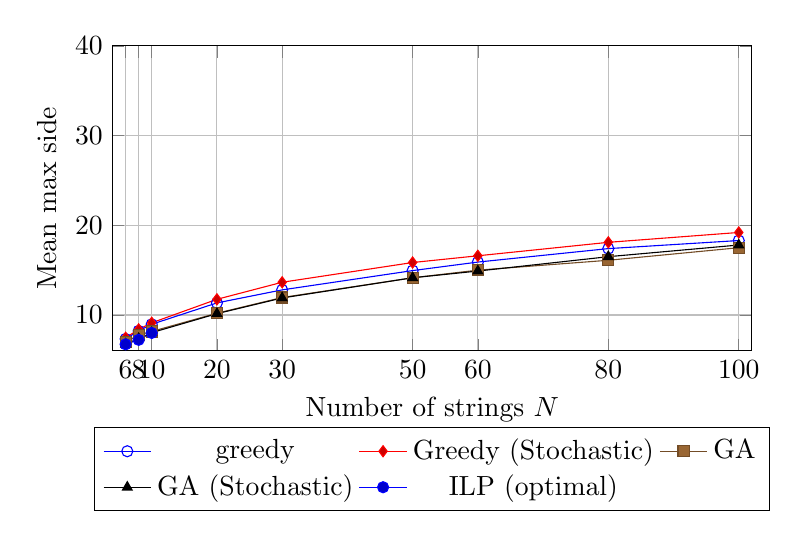
\begin{tikzpicture}
\begin{axis}[
    width=0.8\linewidth,
    height=0.45\linewidth,
    xlabel={Number of strings $N$},
    ylabel={Mean max side},
    xmin=4, xmax=102,
    ymin=6, ymax=40,
    xtick={6,8,10,20,30,50,60,80,100},
    ymajorgrids=true,
    xmajorgrids=true,
    legend style={at={(0.5,-0.25)},anchor=north,legend columns=3},
]
\addplot+[mark=o] coordinates {
  (6,7.3333) (8,8.2333) (10,8.9667)
  (20,11.35) (30,12.8) (50,14.95)
  (60,15.9) (80,17.4) (100,18.3)
};
\addlegendentry{greedy}

\addplot+[mark=diamond*] coordinates {
  (6,7.4667) (8,8.4) (10,9.1333)
  (20,11.75) (30,13.65) (50,15.85)
  (60,16.6) (80,18.1) (100,19.2)
};
\addlegendentry{Greedy (Stochastic)}

\addplot+[mark=square*] coordinates {
  (6,7.0) (8,7.7667) (10,8.1667)
  (20,10.2) (30,11.95) (50,14.15)
  (60,15.0) (80,16.1) (100,17.5)
};
\addlegendentry{GA}

\addplot+[mark=triangle*] coordinates {
  (6,6.7667) (8,7.3667) (10,8.0333)
  (20,10.15) (30,11.9) (50,14.15)
  (60,14.9) (80,16.5) (100,17.8)
};
\addlegendentry{GA (Stochastic)}

\addplot+[mark=*] coordinates {
  (6,6.7333) (8,7.2333) (10,8.0)
};
\addlegendentry{ILP (optimal)}

\end{axis}
\end{tikzpicture}
\caption{Square objective: mean max side vs.\ number of strings. The ILP provides optimal ground truth for $N \le 10$.}
\label{fig:square-cost-vs-tiles}
\end{figure}

\begin{figure}[t]
\centering
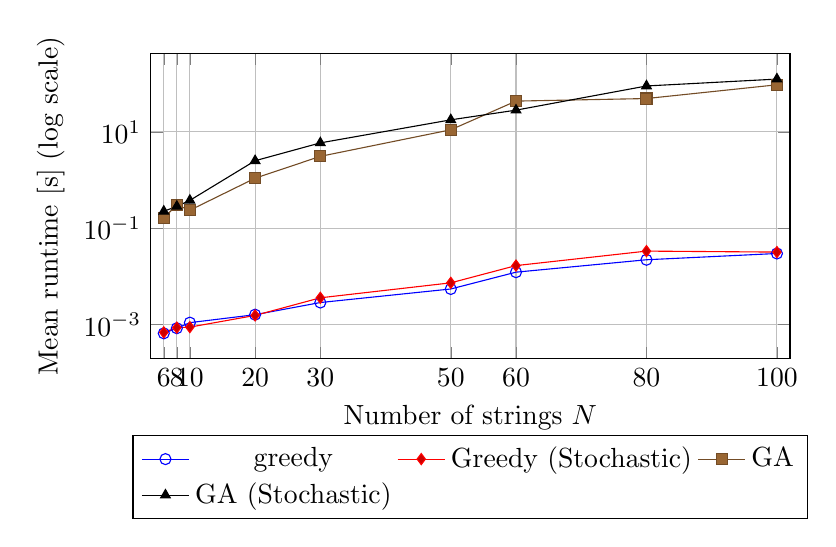
\begin{tikzpicture}
\begin{axis}[
    width=0.8\linewidth,
    height=0.45\linewidth,
    xlabel={Number of strings $N$},
    ylabel={Mean runtime [s] (log scale)},
    xmin=4, xmax=102,
    ymode=log,
    xtick={6,8,10,20,30,50,60,80,100},
    ymajorgrids=true,
    xmajorgrids=true,
    legend style={at={(0.5,-0.25)},anchor=north,legend columns=3},
]
\addplot+[mark=o] coordinates {
  (6,0.0006645) (8,0.0008485) (10,0.0011074)
  (20,0.0016184) (30,0.0028920) (50,0.0055241)
  (60,0.0123243) (80,0.0222861) (100,0.0300579)
};
\addlegendentry{greedy}

\addplot+[mark=diamond*] coordinates {
  (6,0.0006966) (8,0.0008737) (10,0.0008938)
  (20,0.0015631) (30,0.0036246) (50,0.0074041)
  (60,0.0168720) (80,0.0336874) (100,0.0321508)
};
\addlegendentry{Greedy (Stochastic)}

\addplot+[mark=square*] coordinates {
  (6,0.1645) (8,0.3043) (10,0.2369)
  (20,1.0927) (30,3.1055) (50,11.0334)
  (60,43.4149) (80,49.0693) (100,94.6147)
};
\addlegendentry{GA}

\addplot+[mark=triangle*] coordinates {
  (6,0.2254) (8,0.2851) (10,0.3796)
  (20,2.5201) (30,5.9062) (50,17.7508)
  (60,28.1970) (80,89.3945) (100,124.2279)
};
\addlegendentry{GA (Stochastic)}

\end{axis}
\end{tikzpicture}
\caption{Square objective: mean runtime vs.\ number of strings (logarithmic scale) for the heuristic methods.}
\label{fig:square-time-vs-tiles}
\end{figure}

These plots highlight a clear Pareto frontier:
\begin{itemize}
  \item \textsc{greedy} and \textsc{Greedy (Stochastic)} offer the best
        speed--accuracy trade-off when tight time budgets are required.
  \item \textsc{GA} and \textsc{GA (Stochastic)} consistently
        improve the bounding-box side length by roughly $6$--$12\%$ over greedy
        once $N \ge 20$, at the cost of two to three orders of magnitude more
        runtime.
  \item The ILP (\textsc{cplex}) provides verified optimal solutions on small instances ($N \le 10$)
        but is computationally intractable beyond this regime.
\end{itemize}

\subsection{Results for the area objective}
\label{subsec:area-results}

We now turn to the area-based objective $f_{\mathrm{area}}(p) = W(p) \cdot H(p)$, which is the direct 2D analogue of classical superstring length. Tables~\ref{tab:small-results}--\ref{tab:large-results} summarize the average placement cost for each algorithm, grouped by instance scale. Figure~\ref{fig:cost-vs-2Dstrings} visualizes the scaling behavior across all instance sizes.

On small instances (6--10 strings, Table~\ref{tab:small-results}), the ILP provides optimal solutions with mean cost $7.32$, serving as ground truth. The genetic variants are very close to optimal: \textsc{GA (Stochastic)} and \textsc{GA} are only about $2.3\%$ and $4.2\%$ worse than the optimum, respectively. The purely greedy heuristics sacrifice about $12$--$14\%$ in solution quality compared to optimal.

\begin{table}[t]
\centering
\small
\resizebox{0.65\columnwidth}{!}{%
\begin{tabular}{lrrr}
\toprule
Algorithm & Mean cost & Std. dev. \\
\midrule
cplex (optimal)     & 7.32 & 0.63 \\
GA     & 7.63 & 0.63 \\
GA (Stochastic) & 7.49 & 0.67 \\
greedy              & 8.24 & 0.85 \\
Greedy (Stochastic)  & 8.32 & 0.91 \\
\bottomrule
\end{tabular}
}
\caption{Average placement cost on small string sets (6--10 strings), area-based objective. The ILP provides optimal solutions for verification; runtime is omitted as it is used only for offline ground-truth generation.}
\label{tab:small-results}
\end{table}

On medium instances (20--50 strings, Table~\ref{tab:medium-results}), \textsc{GA (Stochastic)} attains the lowest average cost, with \textsc{GA} being essentially indistinguishable (within $0.1\%$). The greedy baselines are roughly $8\%$ (\textsc{greedy}) and $11.5\%$ (\textsc{Greedy (Stochastic)}) worse in cost.

\begin{table}[t]
\centering
\small
\resizebox{0.65\columnwidth}{!}{%
\begin{tabular}{lrr}
\toprule
Algorithm & Mean cost & Std. dev. \\
\midrule
GA     & 12.17 & 1.63 \\
GA (Stochastic) & 12.16 & 1.73 \\
greedy              & 13.17 & 1.76 \\
Greedy (Stochastic)  & 13.56 & 1.77 \\
\bottomrule
\end{tabular}
}
\caption{Average placement cost on medium string sets (20--50 strings), area-based objective.}
\label{tab:medium-results}
\end{table}

On large instances (60--100 strings, Table~\ref{tab:large-results}), \textsc{GA} consistently achieves the best average cost. The cost gap between the GA and the deterministic greedy baseline is around $6$--$7\%$ on average, and around $11\%$ for \textsc{Greedy (Stochastic)}.

\begin{table}[t]
\centering
\small
\resizebox{0.6\columnwidth}{!}{%
\begin{tabular}{lrr}
\toprule
Algorithm & Mean cost & Std. dev. \\
\midrule
GA     & 16.23 & 1.09 \\
GA (Stochastic) & 16.54 & 1.21 \\
greedy              & 17.28 & 1.25 \\
Greedy (Stochastic)  & 18.12 & 1.34 \\
\bottomrule
\end{tabular}
}
\caption{Average placement cost on large string sets (60--100 strings), area-based objective.}
\label{tab:large-results}
\end{table}

\begin{figure}[t]
\centering
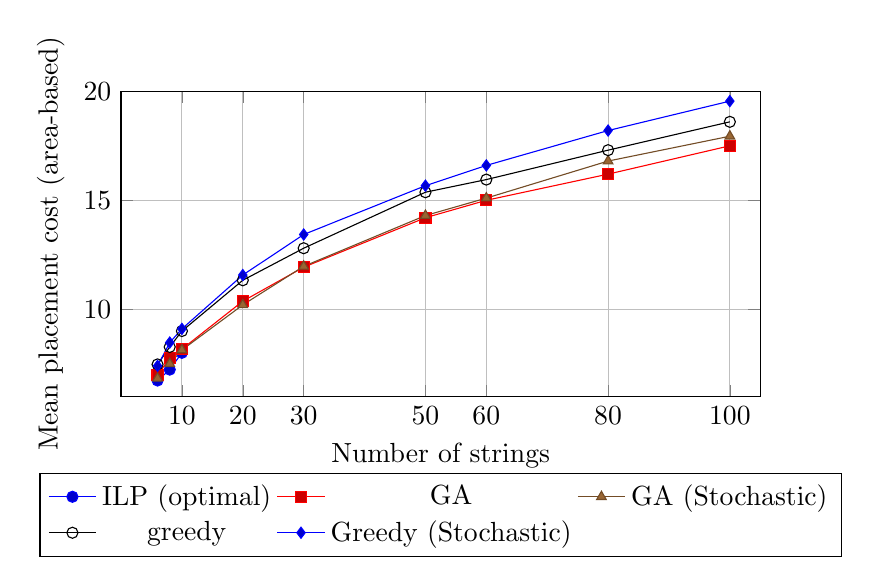
\begin{tikzpicture}
\begin{axis}[
    width=0.8\linewidth,
    height=0.45\linewidth,
    xlabel={Number of strings},
    ylabel={Mean placement cost (area-based)},
    xmin=0, xmax=105,
    ymin=6, ymax=20,
    xtick={10,20,30,50,60,80,100},
    ymajorgrids=true,
    xmajorgrids=true,
    legend style={at={(0.5,-0.25)},anchor=north,legend columns=3},
]
\addplot+[mark=*] coordinates {
  (6,6.73) (8,7.23) (10,8.00)
};
\addlegendentry{ILP (optimal)}

\addplot+[mark=square*] coordinates {
  (6,6.97) (8,7.77) (10,8.17) (20,10.37) (30,11.93) (50,14.20) (60,15.00) (80,16.20) (100,17.50)
};
\addlegendentry{GA}

\addplot+[mark=triangle*] coordinates {
  (6,6.83) (8,7.50) (10,8.13) (20,10.20) (30,11.97) (50,14.30) (60,15.10) (80,16.80) (100,17.94)
};
\addlegendentry{GA (Stochastic)}

\addplot+[mark=o] coordinates {
  (6,7.47) (8,8.27) (10,9.00) (20,11.33) (30,12.80) (50,15.37) (60,15.95) (80,17.30) (100,18.60)
};
\addlegendentry{greedy}

\addplot+[mark=diamond*] coordinates {
  (6,7.40) (8,8.47) (10,9.10) (20,11.57) (30,13.43) (50,15.67) (60,16.60) (80,18.20) (100,19.55)
};
\addlegendentry{Greedy (Stochastic)}

\end{axis}
\end{tikzpicture}
\caption{Mean placement cost (area-based objective) as a function of the number of strings. Each point averages over all random instances for the corresponding size.}
\label{fig:cost-vs-2Dstrings}
\end{figure}

\subsection{Scaling with the number of strings}

To better understand the scaling behaviour, Figures~\ref{fig:cost-vs-2Dstrings} and \ref{fig:time-vs-2Dstrings} plot the mean cost and mean runtime as a function of the number of strings, again using the area-based objective.

Figure~\ref{fig:cost-vs-2Dstrings} shows that for all algorithms the placement cost grows roughly monotonically with the number of strings, as expected. At every size for which optimal solutions are available ($N \le 10$), the ILP provides the ground truth, and the GA variants remain within $2\%$ of the optimum. For larger instances where the ILP is intractable, the GA consistently achieves the best cost. Both greedy baselines trail the best method by between $6\%$ and $14\%$, with an average gap of approximately $7.7\%$ (\textsc{greedy}) and $11.8\%$ (\textsc{Greedy (Stochastic)}) for string sets of size $20$ and larger.

Figure~\ref{fig:time-vs-2Dstrings} (note the logarithmic y-axis) highlights the trade-off between solution quality and runtime for the heuristic methods. The two greedy algorithms are extremely fast and scale almost linearly in the number of strings, remaining below $0.5$ seconds for up to 10 strings and below $3.5$ seconds even at 100 strings. The GA variants incur one to two orders of magnitude more CPU time, with runtime growing from roughly $4$ seconds on 6--10 strings to around $170$--$225$ seconds at 100 strings.

Overall, the experiments suggest a clear Pareto frontier: greedy heuristics provide very fast but moderately suboptimal solutions, while the tree-based genetic algorithms consistently improve the placement cost by roughly $6$--$12\%$ at the expense of significantly higher runtime. Crucially, when verified against optimal ILP solutions on small instances, the GA achieves near-optimal quality, validating its effectiveness on larger instances where ground truth is unavailable.

\begin{figure}
\centering
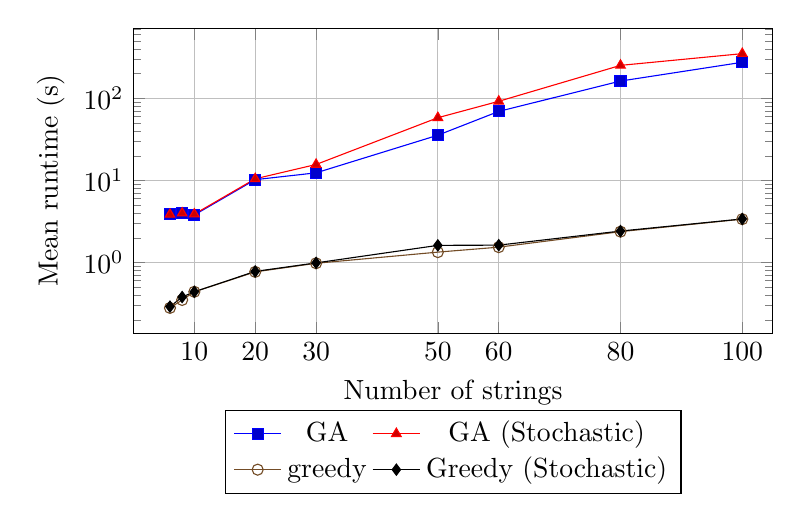
\begin{tikzpicture}
\begin{axis}[
    width=0.8\linewidth,
    height=0.45\linewidth,
    xlabel={Number of strings},
    ylabel={Mean runtime (s)},
    xmin=0, xmax=105,
    ymode=log,
    xtick={10,20,30,50,60,80,100},
    ymajorgrids=true,
    xmajorgrids=true,
    legend style={at={(0.5,-0.25)},anchor=north,legend columns=2},
]

\addplot+[mark=square*] coordinates {
  (6,3.92) (8,4.01) (10,3.80) (20,10.24) (30,12.40) (50,35.66) (60,69.54) (80,163.00) (100,276.00)
};
\addlegendentry{GA}

\addplot+[mark=triangle*] coordinates {
  (6,3.86) (8,4.00) (10,3.89) (20,10.49) (30,15.68) (50,58.26) (60,92.34) (80,253.13) (100,351.74)
};
\addlegendentry{GA (Stochastic)}

\addplot+[mark=o] coordinates {
  (6,0.28) (8,0.35) (10,0.44) (20,0.77) (30,0.98) (50,1.34) (60,1.54) (80,2.38) (100,3.38)
};
\addlegendentry{greedy}

\addplot+[mark=diamond*] coordinates {
  (6,0.29) (8,0.38) (10,0.44) (20,0.78) (30,0.99) (50,1.62) (60,1.63) (80,2.42) (100,3.40)
};
\addlegendentry{Greedy (Stochastic)}

\end{axis}
\end{tikzpicture}
\caption{Mean runtime as a function of the number of strings (logarithmic scale) for the heuristic methods. Greedy heuristics are one to two orders of magnitude faster than the genetic algorithms.}
\label{fig:time-vs-2Dstrings}
\end{figure}

\subsection{Genetic algorithm dynamics and crossover statistics}

To better understand how the genetic algorithms construct their solutions, we instrument \textsc{GA} and \textsc{GA (Stochastic)} with additional counters. For each run we record:
\begin{itemize}
  \item the total number of crossover operations, $C$ (\texttt{total\_crossovers});
  \item the number of crossovers that produce an incomplete placement and therefore require greedy completion, $C_{\text{repair}}$ (\texttt{crossovers\_needing\_completion});
  \item the total number of strings that are finally placed by the greedy completion step across all incomplete offspring, $T_{\text{fix}}$ (\texttt{total\_strings\_completed}).
\end{itemize}

From these quantities we derive:
\begin{align*}
  r_{\text{repair}}
    &= \frac{C_{\text{repair}}}{C}
    && \parbox[t]{.51\linewidth}{%
        repair rate: fraction of crossovers that need greedy fix} \\[4pt]
  \rho_{\text{greedy}}
    &= \frac{T_{\text{fix}}}{C n}
    && \parbox[t]{.51\linewidth}{%
        share of string placements coming from greedy completion} \\[4pt]
  \rho_{\text{direct}}
    &= 1 - \rho_{\text{greedy}}
    && \parbox[t]{.51\linewidth}{%
        ``completion rate'': share of strings placed directly by crossover} \\[4pt]
  \bar{t}_{\text{repair}}
    &= \frac{T_{\text{fix}}}{C_{\text{repair}}}
    && \parbox[t]{.51\linewidth}{%
        average \#missing strings per repaired offspring}.
\end{align*}

\begin{table*}[!t]
\centering
\small
\resizebox{\linewidth}{!}{%
\begin{tabular}{cccccc}
\toprule
Algorithm & Scale & Mean \#crossovers & Repair rate $r_{\text{repair}}$ & Direct strings $\rho_{\text{direct}}$ & Avg.\ strings/repair $\bar{t}_{\text{repair}}$ \\
\midrule
    GA    & small  &  3\,152 &  9.2\% & 97.0\% &   3.0 \\
    GA    & medium & 12\,594 &  6.7\% & 97.0\% &  22.6 \\
    GA    & large  & 28\,357 &  3.1\% & 97.5\% &  68.3 \\
GA (Stochastic)    & small  &  3\,151 & 12.8\% & 95.9\% &   2.7 \\
GA (Stochastic)    & medium & 12\,602 &  8.9\% & 95.2\% &  22.0 \\
GA (Stochastic)    & large  & 28\,354 &  6.3\% & 96.1\% &  60.8 \\
\bottomrule
\end{tabular}
}
\caption{Internal statistics of the genetic algorithms. ``Direct strings'' is the fraction of string placements coming directly from crossover ($\rho_{\text{direct}} = 1 - \rho_{\text{greedy}}$); the remainder are filled by the greedy completion procedure. All experiments here use the area-based objective.}
\label{tab:ga-internals}
\end{table*}

Several trends are apparent:
\begin{itemize}
  \item The number of crossovers per run grows with instance size. On small instances each GA performs about $3.1 \times 10^3$ crossovers; this increases to roughly $1.26 \times 10^4$ on medium instances and $2.8 \times 10^4$ on large instances.
  \item The repair rate $r_{\text{repair}}$ is modest: between $3\%$ and $13\%$ of crossovers produce offspring that are not complete placements. The \textsc{GA (Stochastic)} variant tends to trigger repairs slightly more often than \textsc{GA}.
  \item At the string level, only a very small fraction of the solution is delegated to the greedy completion phase. Across all scales and both GA variants, the mean $\rho_{\text{greedy}}$ is about $3.6\%$, so approximately $96\%$ of string placements come directly from crossover. In other words, the GA's recombination operators are doing almost all of the constructive work.
  \item When a repair is needed, it can be substantial on large instances: on small instances, an incomplete offspring is missing on average $3$ strings out of $8$; on medium instances, around $22$ out of $33$ strings; and on large instances, around $61$--$68$ out of roughly $80$ strings. This reflects the increasing difficulty of producing fully consistent placements purely by recombination when the search space grows.
\end{itemize}

Figure~\ref{fig:crossovers-vs-2Dstrings} plots the average number of crossovers per run as a function of the number of strings. As expected from the fixed population size and generation budget in our implementation, the curves are piecewise constant: roughly $3{,}150$ crossovers for 6--10 strings, $12{,}600$ for 20--50 strings, and $28{,}350$ for 60--100 strings. The two GA variants behave almost identically in this respect.

\begin{figure}
\centering
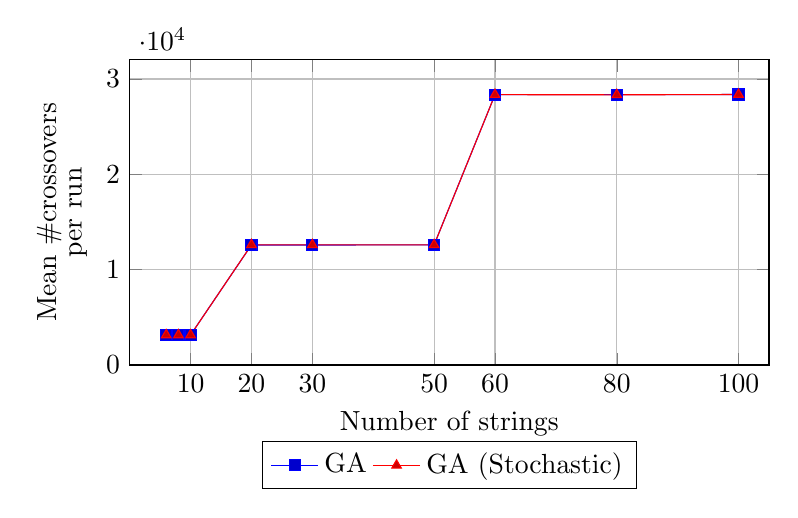
\begin{tikzpicture}
\begin{axis}[
    width=0.8\linewidth,
    height=0.45\linewidth,
    xlabel={Number of strings},
    ylabel={\shortstack{Mean \#crossovers\\per run}},
    xmin=0, xmax=105,
    ymin=0, ymax=32000,
    xtick={10,20,30,50,60,80,100},
    ytick={0,10000,20000,30000},
    ymajorgrids=true,
    xmajorgrids=true,
    legend style={at={(0.5,-0.25)},anchor=north,legend columns=2},
]
\addplot+[mark=square*] coordinates {
  (6,3152.1) (8,3147.1) (10,3157.5) (20,12591.9) (30,12584.2) (50,12606.7) (60,28351.2) (80,28352.5) (100,28367.7)
};
\addlegendentry{GA}

\addplot+[mark=triangle*] coordinates {
  (6,3151.7) (8,3152.4) (10,3148.0) (20,12606.3) (30,12598.7) (50,12601.0) (60,28355.4) (80,28337.5) (100,28370.4)
};
\addlegendentry{GA (Stochastic)}

\end{axis}
\end{tikzpicture}
\caption{Average number of crossovers per run as a function of the number of strings.}
\label{fig:crossovers-vs-2Dstrings}
\end{figure}

Figure~\ref{fig:greedy-share-vs-2Dstrings} focuses on the string-level interaction between crossover and greedy repair by plotting $\rho_{\text{greedy}}$ (the fraction of strings placed by the greedy completion step) as a function of the number of strings. For both GA variants this fraction remains between roughly $2\%$ and $7\%$ across all sizes, confirming that the vast majority of strings in the final placements are produced by crossover rather than by the repair heuristic.

\begin{figure}
\centering
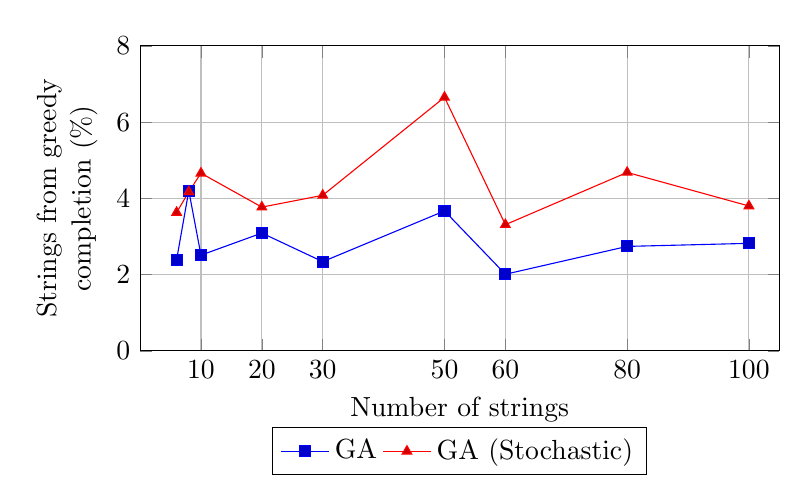
\begin{tikzpicture}
\begin{axis}[
    width=0.8\linewidth,
    height=0.45\linewidth,
    xlabel={Number of strings},
    ylabel={\shortstack{Strings from greedy\\completion (\%)}},
    xmin=0, xmax=105,
    ymin=0, ymax=8,
    xtick={10,20,30,50,60,80,100},
    ytick={0,2,4,6,8},
    ymajorgrids=true,
    xmajorgrids=true,
    legend style={at={(0.5,-0.25)},anchor=north,legend columns=2},
]
\addplot+[mark=square*] coordinates {
  (6,2.39) (8,4.20) (10,2.51) (20,3.09) (30,2.34) (50,3.67) (60,2.01) (80,2.74) (100,2.82)
};
\addlegendentry{GA}

\addplot+[mark=triangle*] coordinates {
  (6,3.63) (8,4.17) (10,4.66) (20,3.77) (30,4.08) (50,6.65) (60,3.31) (80,4.68) (100,3.80)
};
\addlegendentry{GA (Stochastic)}

\end{axis}
\end{tikzpicture}
\caption{Share of string placements produced by the greedy completion step as a function of the number of strings. The complement to $100\%$ can be interpreted as the ``completion rate'' of the crossover operators.}
\label{fig:greedy-share-vs-2Dstrings}
\end{figure}

Taken together, these diagnostics indicate that the GA operates in a regime where (i) crossover is the dominant constructive mechanism, responsible for more than $95\%$ of string placements, and (ii) greedy completion acts as a lightweight but essential repair operator that corrects the relatively small fraction of offspring that violate feasibility, especially on large instances where missing strings can be numerous.

\section{Conclusion}
\label{sec:conclusion}

We have formulated a two-dimensional version of the Shortest Superstring
Problem, in which the goal is to place strings on the integer grid with
symbol-consistent overlaps while optimizing a bounding-box objective derived
from the minimal axis-aligned rectangle containing all occupied cells. We
considered two natural cost variants: a \emph{square} objective, minimizing the
side length $\max\{H,W\}$ of the smallest enclosing square, and an \emph{area}
objective, minimizing the rectangle area $H\cdot W$.

Our work makes three primary contributions:
\begin{enumerate}
    \item \emph{Problem formalization.} We introduce the 2D-SSP as a natural two-dimensional generalization of the classical SSP, with two bounding-box cost variants. We establish the equivalence between optimizing over 2D-superstrings and optimizing over symbol-consistent placements.
    
    \item \emph{Structural theory.} We develop a placement-tree representation that encodes solutions as trees of relative offsets rather than raw 2D arrays. Under mild connectivity assumptions, we prove that optimal solutions admit such tree-based representations and that every feasible placement tree induces a valid solution.
    
    \item \emph{Algorithmic framework.} We develop three algorithmic approaches---an exact ILP formulation, a fast greedy heuristic, and a problem-specific tree-based genetic algorithm---that exploit the placement-tree structure. The GA achieves near-optimal quality with substantially lower runtime than ILP and $6$--$12\%$ better quality than greedy on medium and large instances.
\end{enumerate}

Several limitations of the current work merit discussion. First, our ILP formulation, while exact, does not scale beyond small instances ($n \le 10$ strings) due to the combinatorial explosion of candidate placements. Second, the connectivity assumption (Assumption~\ref{ass:connected-union}) excludes instances where optimal solutions consist of disconnected components. Third, our experimental evaluation uses only $3 \times 3$ strings over small alphabets; the behavior on larger or more varied string shapes remains unexplored. Finally, the GA's performance depends on parameter choices (population size, crossover rate) that we have not systematically tuned.

Several directions for future research emerge from this work:
\begin{itemize}
    \item \emph{Approximation algorithms.} Can the greedy $2.5$-approximation for 1D-SSP be generalized to the 2D setting? What approximation ratios are achievable for 2D-SSP?
    
    \item \emph{Hardness results.} Establishing the precise computational complexity of 2D-SSP (NP-hardness, APX-hardness, or inapproximability bounds) remains open.
    
    \item \emph{Alternative objectives.} Beyond bounding-box cost, one could minimize the total area of the union $|R(p)|$ or consider weighted combinations of area and perimeter.
    
    \item \emph{Rotations and reflections.} Allowing strings to be rotated or reflected would significantly expand the solution space and potentially improve compression ratios.
    
    \item \emph{Applications.} The placement-tree perspective may transfer to related problems in VLSI floorplanning, texture synthesis, and DNA tile assembly where local overlap consistency is central.
\end{itemize}

More broadly, the placement-tree representation and tree-based GA operators developed here may serve as a template for other two-dimensional placement and tiling problems where local overlap structure plays a central role.


\begin{figure*}[!htb]
  \centering
  \resizebox{\textwidth}{!}{%
    \begin{tabular}{l cc cc cc cc cc }
    \toprule[1pt]
    & \multicolumn{2}{c}{CPLEX} & \multicolumn{2}{c}{Greedy} & \multicolumn{2}{c}{Stoch. Greedy} & \multicolumn{2}{c}{Genetic Greedy} & \multicolumn{2}{c}{Genetic Stoch.} \\
    \cmidrule(lr){2-3}\cmidrule(lr){4-5}\cmidrule(lr){6-7}\cmidrule(lr){8-9}\cmidrule(lr){10-11}
    Tiles & Obj & Time & Obj & Time & Obj & Time & Obj & Time & Obj & Time \\
    \midrule[1pt]
    6   & \textbf{6.73} & 2.32   & 7.47 & \textbf{0.28} & 7.40 & 0.29 & 6.97 & 3.92 & 6.83 & 3.86 \\
    8   & \textbf{7.23} & 12.13  & 8.27 & \textbf{0.35} & 8.47 & 0.38 & 7.77 & 4.01 & 7.50 & 4.00 \\
    10  & \textbf{8.00} & 43.88  & 9.00 & \textbf{0.44} & 9.10 & 0.44 & 8.17 & 3.80 & 8.13 & 3.89 \\
    20  & - & - & 11.33 & \textbf{0.77} & 11.57 & 0.78 & 10.37 & 10.24 & \textbf{10.20} & 10.49 \\
    30  & - & - & 12.80 & \textbf{0.98} & 13.43 & 0.99 & \textbf{11.93} & 12.40 & 11.97 & 15.68 \\
    50  & - & - & 15.37 & \textbf{1.34} & 15.67 & 1.62 & \textbf{14.20} & 35.66 & 14.30 & 58.26 \\
    60  & - & - & 15.95 & \textbf{1.54} & 16.60 & 1.63 & \textbf{15.00} & 69.54 & 15.10 & 92.34 \\
    80  & - & - & 17.30 & \textbf{2.38} & 18.20 & 2.42 & \textbf{16.20} & 163.00 & 16.80 & 253.13 \\
    100 & - & - & 18.60 & \textbf{3.38} & 19.55 & 3.40 & \textbf{17.50} & 276.00 & 17.94 & 351.74 \\
    \bottomrule[1pt]
    \end{tabular}
  }
  \caption{Performance comparison across varying number of tiles. CPLEX provides optimal baselines for small scales (Tiles $\le$ 10), while other methods scale to larger instances.}
  \label{fig:tiles_comparison}
\end{figure*}


\begin{figure}[H] 
    \centering
    \includegraphics[width=1.0\linewidth]{figure/compare.png}
    \caption{Comparison of objective values across Small, Medium, and Large scales. The blue bars highlight the best-performing algorithm in each category.}
    \label{fig:objective_comparison}
\end{figure}


% ===================== BACK MATTER =====================

%% Bibliography - Harvard style for Computers & Operations Research
\bibliographystyle{elsarticle-harv}
\bibliography{references}

\end{document}